\documentclass[11pt,a4paper]{ivoa}
\input tthdefs
% widen up the display a bit so that 75 column listings still fit on
% the page
\usepackage[width=14cm,left=4cm]{geometry}
\usepackage{listings}
\lstloadlanguages{XML}
\lstset{flexiblecolumns=true,tagstyle=\ttfamily,showstringspaces=False}
\usepackage{amsmath}

\iftth
\newcommand{\tapschema}{TAP\_SCHE\-MA}
\hyphenation{TAP\_SCHEMA}
\hyphenation{\tapschema}
\newcommand{\tapupload}{TAP\_UPLOAD}
\else
\newcommand{\tapschema}{\mbox{%
  TAP\discretionary{-}{}{\kern-2pt\_}SCHEMA}}
\newcommand{\tapupload}{%
  TAP\discretionary{-}{}{\kern-2pt\_}UPLOAD}
\fi

\title{VODataService: A VOResource Schema Extension for Describing
Collections and Services}

\ivoagroup{Registry}

\author[http://www.ivoa.net/twiki/bin/view/IVOA/RayPlante]{Raymond Plante}
\author[http://www.ivoa.net/twiki/bin/view/IVOA/MarkusDemleitner]{Markus Demleitner}
\author[http://www.ivoa.net/twiki/bin/view/IVOA/AurelienStebe]{Aurélien Stébé}
\author[http://www.ivoa.net/twiki/bin/view/IVOA/KevinBenson]{Kevin Benson}
\author[http://www.ivoa.net/twiki/bin/view/IVOA/PatrickDowler]{Patrick Dowler}
\author[http://www.ivoa.net/twiki/bin/view/IVOA/MatthewGraham]{Matthew Graham}
\author[http://www.ivoa.net/twiki/bin/view/IVOA/GretchenGreene]{Gretchen Greene}
\author[http://www.ivoa.net/twiki/bin/view/IVOA/PaulHarrison]{Paul Harrison}
\author[http://www.ivoa.net/twiki/bin/view/IVOA/GerardLemson]{Gerard Lemson}
\author[http://www.ivoa.net/twiki/bin/view/IVOA/TonyLinde]{Tony Linde}
\author[http://www.ivoa.net/twiki/bin/view/IVOA/GuyRixon]{Guy Rixon}

\editor{Markus Demleitner}
\editor{Ray Plante}

\previousversion[https://ivoa.net/documents/VODataService/20190715/PR-VODataService-1.2-20210223.html]{PR-2021-02-23}
\previousversion[https://ivoa.net/documents/VODataService/20190715/PR-VODataService-1.2-20190715.html]{PR-2019-07-15}
\previousversion[https://ivoa.net/documents/VODataService/20181026/]{WD-2018-10-26}
\previousversion[http://www.ivoa.net/Documents/VODataService/20101202]{REC
1.1}

\begin{document}
\begin{abstract}
VODataService refers to an XML encoding standard for a specialized
extension of the IVOA Resource Metadata that is useful for describing
data collections and the services that access them.  It is defined as
an extension of the core resource metadata encoding standard known as
VOResource \citep{2018ivoa.spec.0625P} using XML Schema.
The specialized resource types defined by the VODataService schema
allow one to describe how the data underlying the resource cover the
sky and the frequency and time axes.
VODataService also enables detailed
descriptions of tables that includes information useful to the
discovery of tabular data.  It is intended that the VODataService data
types will be particularly useful in describing services that support
standard IVOA service protocols.
\end{abstract}

\section*{Acknowledgments}

Versions 1.0 and 1.1 of this document have been developed with support from the
National Science Foundation's
Information Technology Research Program under Cooperative Agreement
AST0122449 with The Johns Hopkins University, from the
UK Particle Physics and Astronomy
Research Council (PPARC), from the European Commission's (EC)
Sixth
Framework Programme via the
Optical Infrared Coordination Network (OPTICON), and from EC's
Seventh Framework Programme
via its
eInfrastructure Science Repositories initiative.

Version 1.2 of this document was developed in part with support from the
German federal ministry for research and education's e-inf-astro project (BMBF
FKZ 05A17VH2).


\section*{Conformance-related definitions}

The words ``MUST'', ``SHALL'', ``SHOULD'', ``MAY'', ``RECOMMENDED'', and
``OPTIONAL'' (in upper or lower case) used in this document are to be
interpreted as described in IETF standard RFC2119 \citep{std:RFC2119}.

The \emph{Virtual Observatory (VO)} is a
general term for a collection of federated resources that can be used
to conduct astronomical research, education, and outreach.
The \href{http://www.ivoa.net}{International
Virtual Observatory Alliance (IVOA)} is a global
collaboration of separately funded projects to develop standards and
infrastructure that enable VO applications.


\section*{Syntax Notation Using XML Schema}

The eXtensible Markup Language, or XML, is a document syntax for marking
textual information with named tags and is defined by \citet{std:XML}.
The set of XML tag names and the syntax
rules for their use is referred to as the document schema.  One way to
formally define a schema for XML documents is using the W3C standard
known as XML Schema \citep{std:XSD}.

The XML Schemas of VODataService as well as VOResource and its other
extensions are
available from the IVOA schema
repository\footnote{\url{http://www.ivoa.net/xml}} at any time.
Parts of the schema appear within the main sections of this document;
however, documentation nodes have been left out for the sake of brevity.
Where the content of the pieces of schema embedded in this text
diverges from the schema document in the IVOA document
repository, the version in the schema repository is authoritative.

References to specific elements and types defined in the VOResource
schema include the namespace prefix \xmlel{vr} as in
\xmlel{vr:Resource} (a type defined in the VOResource schema).

\section{Introduction}

The VOResource standard \citep{2018ivoa.spec.0625P} provides a means of
encoding resource metadata as defined by DataCite \citep{std:DataCite40}
and the VO-specific IVOA Resource Metadata \citep{2007ivoa.spec.0302H} in XML.
VOResource uses XML Schema \citep{std:XSD} to define
most of the XML syntax rules (while a few of the syntax rules are
outside the scope of Schema).  VOResource also describes mechanisms
for creating extensions to the core VOResource metadata.  This allows
for the standardization of new metadata for describing specialized
kinds of resources in a modular way without deprecating the core
schema or other extensions.

This document defines one such extension referred to as VODataService.
It provides types to define data services, their underlying tabular
structures, their service interfaces, and the location of the data
served in space, time, and energy.

The remainder of the document introduces the use cases addressed by this
specification, then provides a high-level overview over the concepts and
usage patterns in sect.~\ref{sect:model} and finally discusses the
concrete classes in sect.~\ref{sect:metadata}.


\subsection{The Role in the IVOA Architecture}

\begin{figure}
\centering
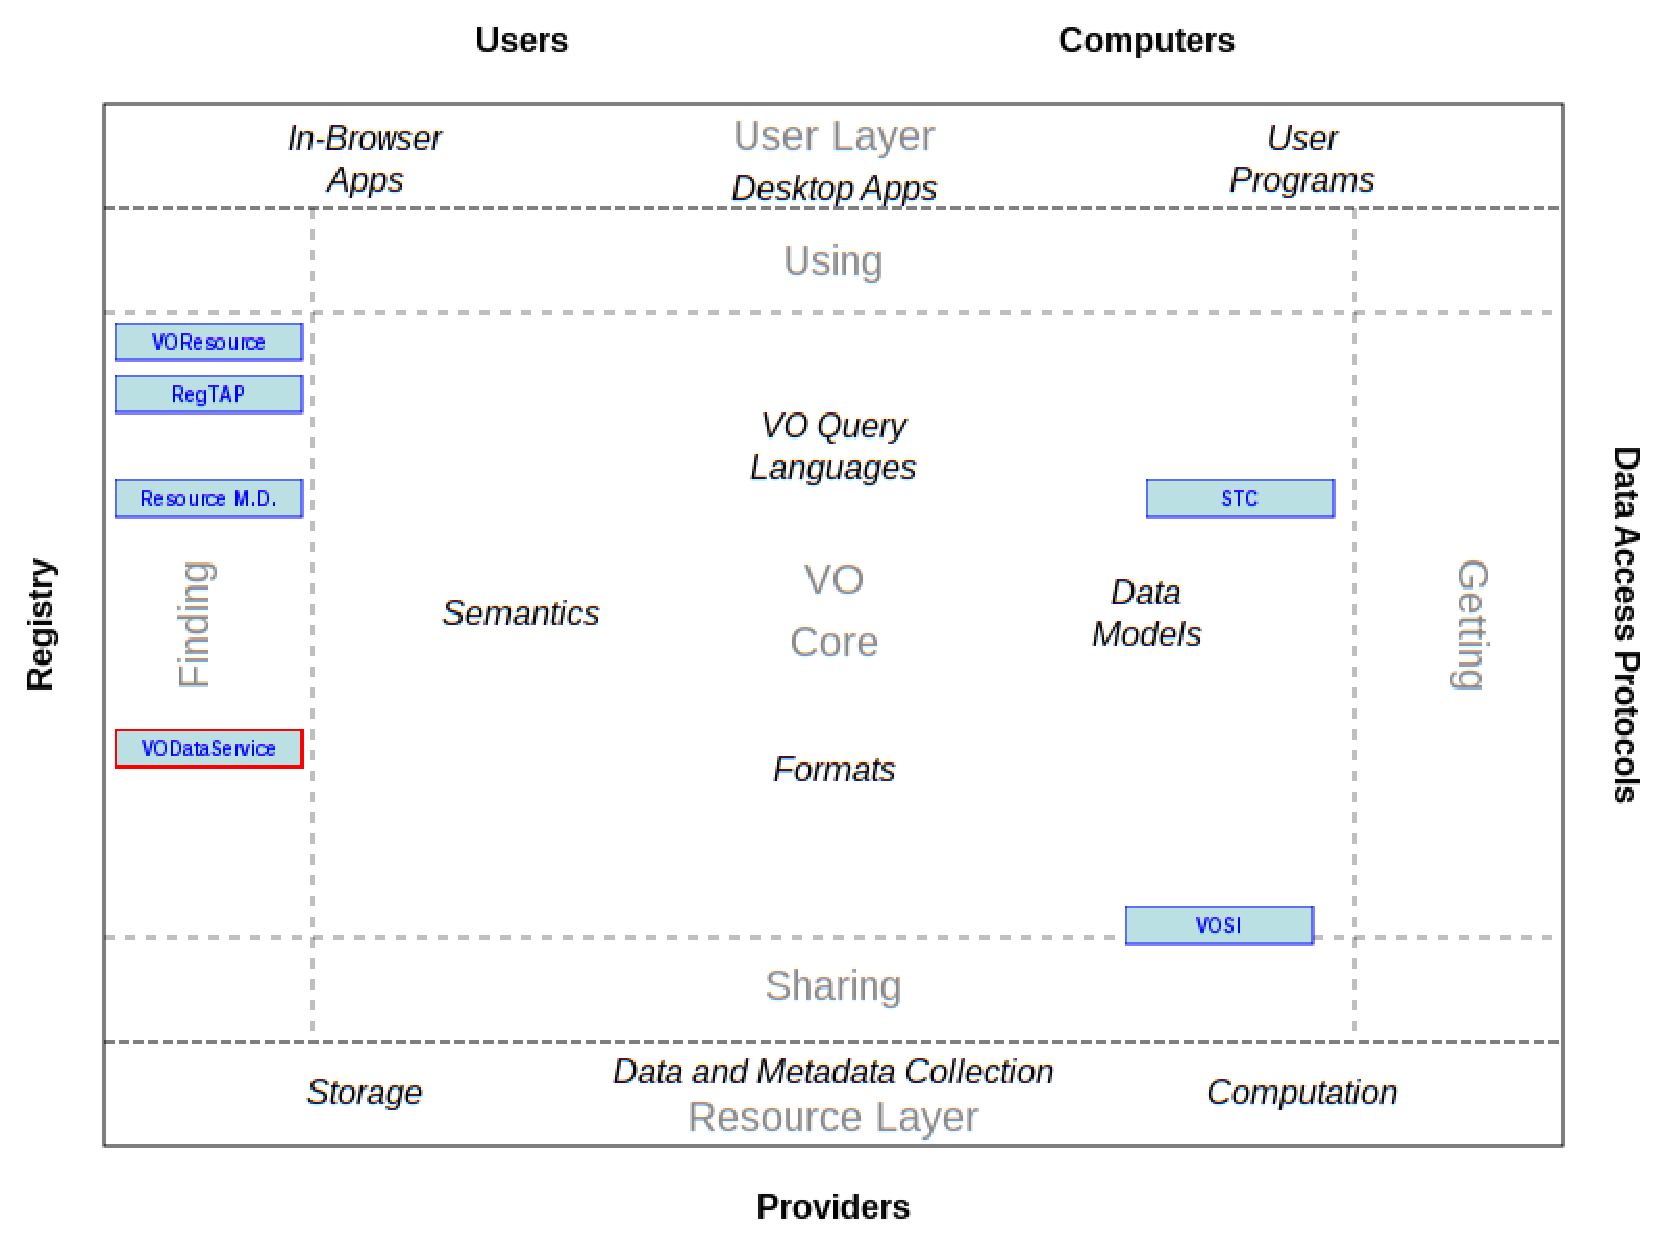
\includegraphics[width=0.9\textwidth]{role_diagram.pdf}
\caption{Architecture diagram for VODataService}
\label{fig:archdiag}
\end{figure}

Fig.~\ref{fig:archdiag} shows the role VODataService plays within the
IVOA Architecture \citep{2010ivoa.rept.1123A}.

VODataService directly depends on the following other VO standards
(unless specified otherwise, the dependency is on the major version of
the cited standard rather than on the exact version):

\begin{description}
\item[VOResource, v1.1 \citep{2018ivoa.spec.0625P}] VOResource gives
the fundamental types and structures extended here.
\item[STC, v1.33 \citep{2007ivoa.spec.1030R}] The deprecated mechanism
for declaring coverage through STCResourceProfile still uses concepts
from version 1 of the IVOA data model for Space-Time Coordinates.  The
updated mechanism has no such dependence any more.
\end{description}

VODataService is closely related to the following other VO standards:

\begin{description}
\item[VOSI, v1.1 \citep{2017ivoa.spec.0524G}] VODataService defines the
schema for the responses on the table metadata endpoint.  It also
defines the ParamHTTP interface type currently used in the capabilities of most
standard protocols.
\item[RegTAP, v1.1 \citep{2019ivoa.spec.1011D}] RegTAP maps the concepts
defined here into a relational structure.  In that sense it is the
user interface to what is specified here.  RegTAP will need an update
to support the space-time constraints added here.
\item[MOC, v1.1 \citep{2019ivoa.spec.1007F}] Multi-Order coverage maps
are used by VODataService to communicate spatial coverage.
\end{description}

\subsection{Purpose}


The purpose of this extension is to define common XML Schema
types -- in particular new resource types -- that are useful for describing
data collections and services that access data.  One aspect of such a
description is the resource's \emph{coverage}:  the parts of the
sky with which the data is associated and the time and frequency ranges that
were observed or modeled to create the data.  Another important aspect
is the detailed metadata for tables underlying the resource, including
names, types, UCDs
\citep{2005ivoa.spec.1231D}, units,
and textual descriptions for the columns making them up.

Resource records using VODataService types are commonly used to register
services that support standard IVOA data access layer protocols such
as Simple Image Access \citep{2015ivoa.spec.1223D} and Simple Cone Search
\citep{2008ivoa.specQ0222P}.  As of October 2018, there are more than
20000~resources of type \xmlel{vs:CatalogService} in the VO Registry.

While other VOResource extensions
define the protocol-specific metadata (encapsulated as a standard
\emph{capability} from VOResource), the general service
resource description shares the common data concepts such as
coverage and tabular data.  Note, however, that a service described
using the VODataService schema need not support any standard
protocols.  With the VODataService extension schema plus the core
VOResource schema, it is possible to describe a custom service
interface that accesses data.



As a legal extension of VOResource, the use
of VODataService is subject to the rules and recommendations for XML
\citep{std:XML}, XML Schema \citep{std:XSD},
and VOResource itself.

\subsection{Additional Use Cases for Version 1.2}

In the following, we collect use cases that guided the development of
VODataService to its version 1.2.  We do not formally derive
requirements from them but briefly note which new features enable or
facilitate the specific use case.

A few of the changes in version 1.2 are necessary for consistency with other standards
such as TAP (extendedType interpretation, requirement to use ADQL
delimited identifier literals in names where appropriate) or VOTable
(arraysize interpretation).  These were obviously not guided by specific
use cases.


\paragraph{What services have data for the Crab nebula covering the
H$\boldsymbol\alpha$
line taken in the second half of 2015?}  In version 1.1, this use case
would have been covered by the \xmlel{stc:STCResourceProfile} type,
which, however, was never properly standardised or widely adopted.  In the current
version, the \xmlel{spatial}, \xmlel{spectral}, and \xmlel{temporal}
children of \xmlel{coverage} enable discovery by coverage on the various
axes.  It is worth noting that the spectral coverage is for the solar
system barycenter, so this use case does \emph{not} immediately enable
the discovery of, say, H$\alpha$ images of remote galaxies.  Redshift
correction has to be applied by the client based on knowledge about the
object(s) investigated.  At the time of writing, coverage also does not
directly address non-celestial reference systems, although in particular
planetary surfaces are considered in scope, and the coverage element's
\xmlel{@frame} attribute is defined to ensure non-ICRS coverages can
safely be declared as the need arises.

\paragraph{Find all ObsCore services publishing data taken at the
Telescope X.} This use case could be satisfied in version 1.1 through
the use of \xmlel{vs:DataCollection} records and relationships to the
respective TAP services.  However, this scheme led to error-prone query
patterns, and few such data collections were actually registered; see
the IVOA Note on discovering data collections \citep{2019ivoa.spec.0520D} for
details.  To better support the scheme proposed there, version 1.2 adds
the \xmlel{vs:DataResource} and \xmlel{vs:CatalogResource} types
that identify a resource as data-like but
permits the addition of various capabilities to the record (which
\xmlel{vs:DataCollection} did not).  An analogous use case would be
``Find all TAP services publishing tables from Gaia DR2''.

\paragraph{Find a large-scale survey of sources between 20 and 40 GHz.}
While the spectral constraint is easily satisfied by the new coverage
children, the ``large-scale'' part is much harder to operationalize.
However, the plain table size often is a useful proxy in such discovery
problems.  The new \xmlel{nrows} child of \xmlel{vs:Table} communicates
it.


\subsection{Additional Use Cases for Future Versions}

The following use cases were originally envisioned for VODataService
1.2, but were postponed because building multiply implemented solutions
for them seemed likely to unnecessarily delay the standardisation of, in
particular, the STC part of the present document.  They will likely be
addressed by future versions of VODataService.

\paragraph{Find a resource that has sources in M51 down to 27 mag in V.}
The constraint about finding a resource that has V magnitudes for M51 is
expressible using spatial coverage and the column's UCDs.  To express
something like ``down to $27^{\rm m}$'' one would at least need
VOTable-style \xmlel{VALUES} children for columns; however, metadata
sufficient to address the next use case would certainly be sufficient
here as well.

\paragraph{Plan a cross-service query.} Systems like OGSA-DAI
\citep{2011ASPC..442..579H} perform orchestration of SQL-like queries
between multiple services automatically, in particular cross-service
JOINs.  In order to work efficiently, such services need column
statistics like histograms and the percentage of NULL values.

\paragraph{Find services serving time series.} In the current registry
model, users looking for spectra would select SSAP services.  With the
growing adoption of ObsCore (and a growing number of services abusing
SSAP to serve time series), the model of selecting data types by
constraining the service protocol no longer works; in the ObsCore
example, clients now have to query all services and constrain the
\verb|dataproduct_type| column. However, for dataset types not overly
common, well more than 90\% of the services could be excluded without
sending a query there based on a declaration of dataset types available
in the Registry.

\paragraph{Facilitate discovery of full DALI services.}  The issue here
is that DALI forsees synchronous and asynchronous endpoints as the
standard case for many protocols -- it already is standard for TAP.
Also, several auxiliary endpoints (mostly defined in VOSI) are declared as
separate capabilities and need to be matched with the functional
endpoints.  This matching is becoming a problem when multiple
authentication schemes or mirror sites necessitate multiple sync/async
pairs.  A longer treatment of this problem has been published while this
document was in WD \citep{note:caproles}, but at the time of writing the
process of finding consensus has just begun, so again a normative
solution has to be deferred to a later version of this standard.



\section{The VODataService Data Model}
\label{sect:model}


The VODataService extension in general enables the description of two
types of resources:  Services that access data on the one side, and data
being accessed through services on the other.

For simple services just publishing a simple resource -- still a fairly
common pattern -- the metadata of the data published can be folded into
the service record.
Here is an example of such a record (abbreviated for the
purposes of illustration) that describes a service from the NASA
Extragalactic Database (NED) that provides measured redshifts for a
given object.


\lstinputlisting[language=XML,basicstyle=\footnotesize,numbers=left]{ipac-resource.xml}

This example illustrates some of the features of the VODataService
extension:

\begin{enumerate}
\item The specific type of resource indicated by
       the value of the \xmlel{xsi:type} attribute; in this case
       \xmlel{vs:CatalogService} indicates that this is
       describing a service that accesses tabular data (line 1).
\item The extra namespace declaration for
       VODataService metadata with the canonical prefix (line 5).
\item The location of the VOResource-related schema
       documents used by this description (line 7ff.)
\item The core VOResource metadata (line 12ff.)
\item An interface described by the
       VODataService type \xmlel{vs:ParamHTTP}; this
       type can indicate input arguments the service supports (line
       40ff.)
\item A description of the
       coverage, including quantitative coverage
       plus waveband keywords (line 62ff.)
\item A description of the table that is returned
       by the service (line 73ff.)
\end{enumerate}

\subsection{The Schema Namespace and Location}


The namespace associated with VODataService extensions is
$$\mbox{\texttt{http://www.ivoa.net/xml/VODataService/v1.1}}.$$
As required by the IVOA schema versioning policies
\citep{2018ivoa.spec.0529H}, this namespace is identical to the one
associated with version 1.1 of this document.  It is regrettable that a
misleading minor version is present in the namespace URI, but dropping
it would break existing software for creating and processing
VODataService instance documents.  Hence, the namespace URI ending in
\verb|1.1| is also used for schema versions 1.2, 1.3, and so forth.

Resolving the VODataService namespace URI will redirect to a schema
document having the actual version number (for the schema associated
with this document version, this will end in VODataService-1.2.xsd).
Following the schema versioning policies, the minor version will be
declared in the \xmlel{version} attribute of this file's root element.
This information should not in general be used in production software;
all versions with the above schema URI are compatible with each
other in the sense defined in the IVOA schema versioning policies.

Authors of VOResource instance documents may choose to
provide a location for the VOResource XML Schema document and its
extensions using the
\xmlel{xsi:schemaLocation} attribute.  While authors are free to
choose a location (as long as it resolves to the schema document), this
specification
recommends using the VODataService namespace URI as its location URL
(as illustrated in the example above), as in
\begin{verbatim}
xsi:schemaLocation="http://www.ivoa.net/xml/VODataService/v1.1
                    http://www.ivoa.net/xml/VODataService/v1.1"
\end{verbatim}

The canonical prefix for VODataService is \xmlel{vs}; this means, in
particular, that in non-XML contexts (e.g., relational mappings
like RegTAP) the VODataService types \emph{must} be qualified with
vs:.

As recommended by the VOResource standard, the
VODataService schema sets \xmlel{element\-Form\-Default} to \emph{unqualified}.
This means that element names defined
in this schema may not be used with a namespace prefix.
The only place the namespace prefix must be used is the
type names given as the value of an
\xmlel{xsi:type} attribute.


\subsection{Summary of Metadata Concepts}
\label{sect:summ}


VODataService defines several resource types and some auxiliary classes
necessary to describe resources of these new types.

\subsubsection{Auxiliary Classes}

The VODataService type \xmlel{vs:Coverage} allows the declaration of
the physical coverage of a resource on the sky (or on spherical bodies),
in time, and in the energy of the messenger particle.  In addition, the
element should contain a rough indication of the messenger type
(e.g., ``Optical''), and it can contain a link to a footprint endpoint and an
indication of the spatial resolution within a service.

VODataService has several classes for the declaration of the tabular
structure underlying a service; this can be the tables in a
TAP-accessible resource,
or it can relate to the data structure returned by the service.  This
metadata is held in
\xmlel{vs:TableSet}-typed elements consisting
of one or more (possibly anonymous)
\xmlel{vs:TableSchema} instances.  These have some very basic metadata
(name, title, description, utype) and otherwise contain \xmlel{vs:Table}
instances.  These in turn have simple metadata, but mainly give column
metadata (including UCDs and units) in \xmlel{vs:TableParam}-typed
children.  These are the basis for enabling discovery queries like
``find all resources having redshifts and far infrared fluxes''.

Note that table and schema metadata is deliberately shallow.  If the
main resource metadata is not enough to discover the table -- as is
fairly typical when a TAP service contains multiple unrelated tables --,
data providers should define separate records for them as described in
sect.~\ref{sect:discoverdata}.

VODataService further defines a specialized interface type
(inheriting from \xmlel{vr:Interface}) called
\xmlel{vs:ParamHTTP}.  This type is used to describe
straightforward HTTP interfaces directly operating on
arguments encoded as
\emph{name=value} pairs.  Such interface declarations can
enumerate a service's input arguments, which enables clients
to generate simple
user interfaces from VOSI capabilities responses.

To be able to express the types of table columns and service arguments
alike, VODataService defines several type systems.  All of these are
basically just enumerations of type names, possibly with some additional
metadata like VOTable-style array sizes.  In new resource records, only
\xmlel{vs:SimpleDataType} (for ParamHTTP parameters on non-DALI
interfaces) and
\xmlel{vs:VOTableType} (for table columns) should be used.

\subsubsection{VODataService Resource Classes}
\label{sect:rescls}

\begin{figure}
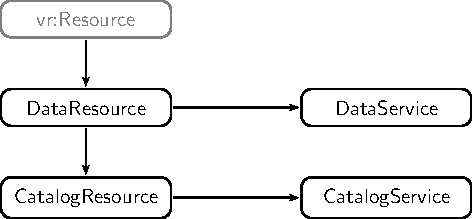
\includegraphics{resclasses.pdf}
\caption{The four major resource classes in VODataService and their
derivation tree}
\label{fig:rescls}
\end{figure}

While no common VO service discovery pattern relies on the XSD type  of the
resource,\footnote{Of course, in non-service discovery (e.g., authorities
or standards), resource types are important.} resource
record authors should
nevertheless choose appropriate types for their resources.  At the
very least, this helps Registry maintenance.

VODataService provides four major resource classes; their derivation
tree is shown in Fig.~\ref{fig:rescls}.  The vertical distinction in
that figure reflects whether a resource has an associated tableset
(DataX vs.~CatalogX); you would typically use the DataX types when a
resource does not naturally admit a relational structure.  The classical
example for this would be a collection of files on an FTP server.  CatalogX,
on the other hand, has an associated tableset.  That does not mean that
it is limited to what is conventionally thought of as a ``catalogue'',
i.e., a table of data on astronomical objects.  On the
contrary, CatalogX should also be used for collections of images,
spectra, time series, etc, as long as their metadata is sufficiently
structured.  That a data collection is published through the standard
IVOA discovery protocols (ObsCore,
SIAP, SSAP) certainly is a strong indication that this requirement is
satisfied.

The horizontal distinction (XResource vs.~XService) is somewhat more
subtle and will be discussed in sect.~\ref{sect:discoverdata}.

Two further resource classes defined VODataService 1.1,
\xmlel{vs:DataCollection} and \xmlel{vs:StandardSTC},
are deprecated in version 1.2.
Resource record authors are requested to migrate or discard resource
records using these deprecated types.  If all such records have
disappeared from the VO by version 1.3 of this specification, their
type declarations may be removed from the schema.

\subsubsection{Discovering Data Within Other Services}
\label{sect:discoverdata}

The content models of CatalogResource and CatalogService are identical.
To understand why the two classes are present nevertheless, a short
historical excursion is in order.  A full treatment of this is found in
the IVOA Endorsed Note on discovering data collections within services
\citep{2019ivoa.spec.0520D}, hereafter referred to as DDC.

In the early VO, there was almost throughout a $1:1$ relationship between
data collections and services.  For instance, a catalogue of variable
stars had a single cone search interface, and the spectra from a given
spectrograph had a single SSA interface.  This is the model reflected by
the CatalogService class, and it was, by and large, sufficient for
IVOA's ``simple'' protocols (SCS, SIAP, SSAP, SLAP), although even these
protocols have facilities for multi-collection services.

With the advent of services very naturally publishing what clearly
are multiple different resources -- TAP, with its multiple tables, and
Obscore building on top of it are the prime examples --, this model
proved inadequate; furthermore, publishers increasingly offered data
through multiple interfaces: An object catalogue now quite typically is
published as both a cone search service and within a TAP service; an
image collection could have both SIAP and Obscore interfaces.

Thus, the relationship between data collections and services gradually
became $n:m$.  With this came the realisation that two classes of
discovery need to be supported; for all-VO queries, validation, and the
like, an enumeration of all \emph{services} (``give me all SSAP
services\dots'') needs to be performed.  For data discovery (``Where are
images from instrument X of object Y?''), a selection over all
\emph{collections} needs to be made.

The solution eventually adopted for these problems is auxiliary
capabilities as introduced in DDC.  They provide stubs merely
identifying an access protocol -- at the same time identifying the
capability as an auxiliary one --  and access URLs, delegating all
further service metadata to a separate record, linked to the original
resource through an \emph{isServedBy} relationship.

Thus, CatalogService-typed records should be used

\begin{itemize}
\item when a service serves a single data collection, in which case the
metadata on the record describes the data collection (e.g., ``These are
observations of\dots'').
\item for a service serving multiple data collections, in which case the
metadata on the record  describes the service (e.g., ``This is the TAP
service of\dots''').
\end{itemize}

CatalogResource-typed records should be used for resources that only
have auxiliary capabilities.

Here is a sketch of a resource record of a table within a TAP service::

\begin{lstlisting}[language=XML,basicstyle=\footnotesize]
<ri:Resource
  xsi:type="vs:CatalogResource"
  <title>Sample Table</title>
  <identifier>ivo://example/sample</identifier>
  <curation>...</curation>
  <content> ...
    <relationship>
      <relationshipType>IsServedBy</relationshipType>
      <relatedResource ivo-id="ivo://example/tap"
        >Example TAP service</relatedResource>
    </relationship>
  </content>
  <capability standardID="ivo://ivoa.net/std/TAP#aux">
    <interface role="std" xsi:type="vs:ParamHTTP">
      <accessURL use="base"
        >http://example.org/svcs/tap</accessURL>
    </interface>
 </capability>
  <coverage>...</coverage>
  <tableset>
    <schema>
      <name>someschema</name>
      <table>
        <name>someschema.sample</name>...
        ...
      </table>
    </schema>
  </tableset>
</ri:Resource>
\end{lstlisting}

A complete example can be found in DDC.

Note that it is legal to add auxiliary capabilities to CatalogService
records as well.  The classical example could be a cone search service
serving a single catalogue that is also queriable within a larger TAP
service.

Analogous considerations would apply to DataResource versus DataService,
although at this point no obvious use cases have been identified;
DataResource was included mainly for symmetry with CatalogResource.

\section{The VODataService Metadata}
\label{sect:metadata}


This section enumerates the types and elements defined in the
VODataService extension schema and describes their meaning.


\subsection{VODataService Resource Types}
\label{sect:resext}

For an overview of the systematics of the following resource types,
please see Sect.~\ref{sect:rescls}.

\subsubsection{DataResource}
\label{sect:DataResource}

The \xmlel{vs:DataResource} resource type is used to describe a
resource containing generic astronomical data without a dominating
tabular structure.  An example might be a largely unstructured archive
of various observations.  Resources that have structured metadata tables
(like most VO services) or are tabular in nature (like usual
astronomical catalogues) should use \xmlel{vs:CatalogResource}.

The type is derived from \xmlel{vr:Service}, which means that instances
can have
capabilities.  For \xmlel{vs:DataResource}, only auxiliary capabilities
(e.g., DataServices serving multiple DataResources) or plain capabilities
with \xmlel{vr:WebBrowser} interfaces should be given.  Resources with a
primary access mode dedicated to the resource's data content should use
\xmlel{vs:DataService}-typed resources.

In addition to \xmlel{vr:Service}'s content, DataResource adds
elements for declaring the observing facilities and/or instruments used
to obtain the data, and it supports the declaration of
the physical coverage of data via the \xmlel{coverage}
element.

% GENERATED: !schemadoc VODataService-v1.2.xsd DataResource
\begin{generated}
\begingroup
      	\renewcommand*\descriptionlabel[1]{%
      	\hbox to 5.5em{\emph{#1}\hfil}}\vspace{2ex}\noindent\textbf{\xmlel{vs:DataResource} Type Schema Documentation}

\noindent{\small
           A resource publishing astronomical data.
         \par}

\noindent{\small
            This resource type should only be used if the resource has no
            common underlying tabular schema (e.g., an inhomogeneous archive).
            Use CatalogResource otherwise.
         \par}

\vspace{1ex}\noindent\textbf{\xmlel{vs:DataResource} Type Schema Definition}

\begin{lstlisting}[language=XML,basicstyle=\footnotesize]
<xs:complexType name="DataResource" >
  <xs:complexContent >
    <xs:extension base="vr:Service" >
      <xs:sequence >
        <xs:element name="facility" type="vr:ResourceName" minOccurs="0"
                  maxOccurs="unbounded" />
        <xs:element name="instrument" type="vr:ResourceName" minOccurs="0"
                  maxOccurs="unbounded" />
        <xs:element name="coverage" type="vs:Coverage" minOccurs="0" />
      </xs:sequence>
    </xs:extension>
  </xs:complexContent>
</xs:complexType>
\end{lstlisting}

\vspace{0.5ex}\noindent\textbf{\xmlel{vs:DataResource} Extension Metadata Elements}

\begingroup\small\begin{bigdescription}\item[Element \xmlel{facility}]
\begin{description}
\item[Type] string with ID attribute: vr:ResourceName
\item[Meaning]
                     The observatory or facility used to collect the data
                     contained or managed by this resource.

\item[Occurrence] optional; multiple occurrences allowed.

\end{description}
\item[Element \xmlel{instrument}]
\begin{description}
\item[Type] string with ID attribute: vr:ResourceName
\item[Meaning]
                     The instrument used to collect the data contain or
                     managed by a resource.

\item[Occurrence] optional; multiple occurrences allowed.

\end{description}
\item[Element \xmlel{coverage}]
\begin{description}
\item[Type] composite: \xmlel{vs:Coverage}
\item[Meaning]
                     Extent of the content of the resource over space, time,
                     and frequency.

\item[Occurrence] optional

\end{description}


\end{bigdescription}\endgroup

\endgroup
\end{generated}

% /GENERATED

\subsubsection{DataService}

The \xmlel{vs:DataService} resource type has the same content model as
\xmlel{vs:DataResource}.  It should be used instead of
\xmlel{vs:DataResource} when the resource's capabilities give
access to (essentially) only the resource's data, as for instance
``ftp service for the XY instrument'', or for a service giving access
to multiple resources; in this latter case, the resource-level
metadata should pertain to the service itself rather than any specific
data collection served by it.

As with \xmlel{vs:CatalogResource}, instances SHOULD
declare the metadata of the table(s) underlying the service or
delivered by it in a \xmlel{tableset} element.

Whenever the service operates on clearly definable tabular
data, the resource should use the \xmlel{vs:CatalogService} resource type
in preference to \xmlel{vs:DataService}, and that tabular structure
should be given in a table set.

DataService's content model is exactly the one of
\xmlel{vs:DataResource}; please refer to sect.~\ref{sect:DataResource}
for the motivation of this duplication.




\subsubsection{CatalogResource}
\label{sect:CatalogResource}


The \xmlel{vs:CatalogResource} resource type is used to describe a
resource containing astronomical data or metadata in a set of one or
more tables.  It extends \xmlel{vs:DataResource} and thus has metadata
on coverage as well as the facilities and instruments that produced the
resource.  Additionally, \xmlel{vs:CatalogResource} instances SHOULD
declare of the metadata of the table(s) making up the data
\xmlel{tableset} element.

As with \xmlel{vs:DataResource}, this type should only be used if all
capabilities declared in the resource are either auxiliary or
nonstandard.  This is typically the case for catalogues or data
collections within larger TAP, ObsTAP, or perhaps SIAP services.  When
a service only publishes a single resource, use the
\xmlel{vs:CatalogService} type.


% GENERATED: !schemadoc VODataService-v1.2.xsd CatalogResource
\begin{generated}
\begingroup
      	\renewcommand*\descriptionlabel[1]{%
      	\hbox to 5.5em{\emph{#1}\hfil}}\vspace{2ex}\noindent\textbf{\xmlel{vs:CatalogResource} Type Schema Documentation}

\noindent{\small
            A resource giving astronomical data in tabular form.
         \par}

\noindent{\small
            While this includes classical astronomical catalogues,
            this resource is also appropriate for collections of observations
            or simulation results provided their metadata are available
            in a sufficiently structured form (e.g., Obscore, SSAP, etc).
         \par}

\vspace{1ex}\noindent\textbf{\xmlel{vs:CatalogResource} Type Schema Definition}

\begin{lstlisting}[language=XML,basicstyle=\footnotesize]
<xs:complexType name="CatalogResource" >
  <xs:complexContent >
    <xs:extension base="vs:DataResource" >
      <xs:sequence >
        <xs:element name="tableset" type="vs:TableSet" minOccurs="0" >
          <xs:unique name="CatalogService-schemaName" >
            <xs:selector xpath="schema" />
            <xs:field xpath="name" />
          </xs:unique>
          <xs:unique name="CatalogService-tableName" >
            <xs:selector xpath="schema/table" />
            <xs:field xpath="name" />
          </xs:unique>
        </xs:element>
      </xs:sequence>
    </xs:extension>
  </xs:complexContent>
</xs:complexType>
\end{lstlisting}

\vspace{0.5ex}\noindent\textbf{\xmlel{vs:CatalogResource} Extension Metadata Elements}

\begingroup\small\begin{bigdescription}\item[Element \xmlel{tableset}]
\begin{description}
\item[Type] composite: \xmlel{vs:TableSet}
\item[Meaning]
                       A description of the tables that are accessible
                       through this service.

\item[Occurrence] optional
\item[Comment]
                     	Each schema name must be unique within a tableset.


\end{description}


\end{bigdescription}\endgroup

\endgroup
\end{generated}

% /GENERATED


\subsubsection{CatalogService}

The \xmlel{vs:CatalogService} resource type is used to describe a
service publishing astronomical data or metadata based on tabular
representations.  Its relationship to \xmlel{vs:CatalogResource}
is as between \xmlel{vs:DataResource}
and \xmlel{vs:DataService}: Use \xmlel{vs:CatalogService} when either
the resource's capabilities are exclusive to the resource described by
the resource-level metadata (``SSAP service for the XY instrument'') or
if the service publishes multiple other CatalogResources; in that latter
case, again, the resource-level metadata should not refer to any
specific data collection contained.

This is the type that should be used for one-resource VO
services.

CatalogService's content model is exactly the one of
\xmlel{vs:CatalogResource}; please refer to sect.~\ref{sect:CatalogResource}
for the motivation of this duplication.

\subsubsection{DataCollection}
\label{sect:datacollection}

The \xmlel{vs:DataCollection} type is deprecated and should no longer be
used in new resource records.  It was used in version 1.1 to define
simple collections of data, much like \xmlel{vs:CatalogResource} in the
current version.  It did not admit capabilities, though, and since the
addition of capabilities would essentially have created a CatalogService
clone with a different child sequence, it was decided to abandon rather
than repair it.

Existing \xmlel{vs:DataCollection}-typed
records should be migrated to records of type \xmlel{vs:DataResource} or
\xmlel{vs:CatalogResource} as appropriate.  If \xmlel{accessURL}
children are present in the
\xmlel{vs:DataCollection}\/s,
they can be replaced with a plain capability with a
\xmlel{vr:WebBrowser}-typed interface.

This type may be removed from the schema when all resource records using
it have vanished from the VO Registry.

\subsubsection{StandardSTC}

The \xmlel{vs:StandardSTC} type is deprecated and should no longer be
used in new resource records.  Since the XML serialisation of the STC 1
data model was never promoted to an IVOA recommendation, there also is
no properly standardised way of creating such records.  Since no such
records ever existed in the Registry, this type will probably be removed
from the schema in version 1.3 of this specification.



\subsection{Coverage in Space, Time, and Spectrum}
\label{sect:cover}

The \xmlel{vs:Coverage} type summarily describes how the data served is
distributed on the
sky, in energy, and in time.

In addition, there is the \xmlel{waveband} element that originally
contained a qualitative indication of the location of the resource's
coverage on the electromagnetic spectrum.  As more resources cover
non-electromagnetic messengers, the element's meaning has somewhat
shifted, and it now admits values from an extendable vocabulary of
messengers\footnote{\url{http://www.ivoa.net/rdf/messenger}} that, for
instance, includes Neutrinos.

Historically, the quantitative footprints were expected to be given in
the element of type \xmlel{stc:STCResourceProfile}\footnote{Defined in
\url{http://www.ivoa.net/xml/STC/stc-v1.30.xsd}}.  As discussed in
\citet{note:regstc}, this expectation turned out to be erroneous,
and the underlying standard, STC-X \citep{note:stcx}, never proceeded to become
a recommendation.  Hence, this version of VODataService deprecates the
use of \xmlel{STCResourceProfile}.

Instead, resource record authors are strongly encouraged to provide
coverage information in the \xmlel{spatial}, \xmlel{spectral}, and
\xmlel{temporal} children of \xmlel{coverage}.

Spatial coverage is conveyed as a MOC.  To enable easy embedding into
resource records written in VOResource (i.e., XML),
VODataService uses the string serialisation defined in section 2.3.2 of
\citet{2019ivoa.spec.1007F}.

By default, the MOCs are to be interpreted in the ICRS.  Future
extensions to non-celestial frames (e.g., on planet
surfaces) will use the \xmlel{frame} attribute.
However, the only celestial reference system allowed is
ICRS.  If a resource's native coordinates are given for another frame (e.g.,
Galactic or FK4 for some equinox), it is the resource record author's
responsibility to convert the spatial coverage into the ICRS.

An important characteristic of MOCs is the order of the smallest scale
(the ``MOC resolution'').  Higher orders yield more faithful
representations of the actual coverage, but also lead to a possibly
significant increase of the size of the serialized MOC.  We suggest a
``typical resolution'' of the Registry of about a degree (i.e., MOC
order 6), but resources are free to choose a higher maximum orders if
appropriate and the resource record size remains reasonable.

Resources that need to communicate high-resolution spatial coverage,
perhaps for some non-discovery use case, can use the \xmlel{footprint}
element with its \xmlel{ivo-id} attribute set to
\nolinkurl{ivo://ivoa.net/std/moc} to declare a URL giving a
footprint in one of the approved MOC serialisations and of arbitrary
level and size.

Time and spectral coverage are modeled as unions of simple
intervals over real numbers; the serialisation here is a space-separated
pair of floating point numbers as governed by the DALI \emph{interval}
xtype.

Times are given in Barycentric Dynamical Time (TDB) at the solar system
barycenter.  They must be specified as Modified Julian Dates.  Since
discovery use cases in which high-precision times are required are not
forseen, resource record authors are encouraged to pad their actual
temporal coverage such that differences in time scales (of the order of
10s of seconds) or reference positions (of the order of minutes between
ground-based observatories and the barycenter) do not matter.  In other
words, the temporal resolution of the Registry at this point should be
assumed to be of order 10 minutes.

Deviating from common VO practice (which currently fairly consistently
uses wavelengths of electromagnetic waves in vacuum), spectral limits are
given in Joules of messenger energy.  This is intended to allow seamless
integration of non-electromagnetic messengers.  The reference position
for the spectral axis is the solar system barycenter.  Again, discovery
use cases on a level where the difference between reference frames of
ground-based observatories versus the solar system barycenter matters
are not forseen, and resource record authors are advised to pad their
intervals on that level.

% GENERATED: !schemadoc VODataService-v1.2.xsd Coverage
\begin{generated}
\begingroup
      	\renewcommand*\descriptionlabel[1]{%
      	\hbox to 5.5em{\emph{#1}\hfil}}\vspace{2ex}\noindent\textbf{\xmlel{vs:Coverage} Type Schema Documentation}

\noindent{\small
           A description of how a resource's contents or behavior maps
           to the sky, to time, and to frequency space, including
           coverage and resolution.
         \par}

\vspace{1ex}\noindent\textbf{\xmlel{vs:Coverage} Type Schema Definition}

\begin{lstlisting}[language=XML,basicstyle=\footnotesize]
<xs:complexType name="Coverage" >
  <xs:sequence >
    <xs:element ref="stc:STCResourceProfile" minOccurs="0" />
    <xs:element name="spatial" type="vs:SpatialCoverage" minOccurs="0" />
    <xs:element name="temporal" type="vs:FloatInterval" minOccurs="0"
              maxOccurs="unbounded" />
    <xs:element name="spectral" type="vs:FloatInterval" minOccurs="0"
              maxOccurs="unbounded" />
    <xs:element name="footprint" type="vs:ServiceReference" minOccurs="0" />
    <xs:element name="waveband" type="xs:token" minOccurs="0"
              maxOccurs="unbounded" />
    <xs:element name="regionOfRegard" type="xs:float" minOccurs="0" />
  </xs:sequence>
</xs:complexType>
\end{lstlisting}

\vspace{0.5ex}\noindent\textbf{\xmlel{vs:Coverage} Metadata Elements}

\begingroup\small\begin{bigdescription}\item[Element \xmlel{stc:STCResourceProfile}]

                 An STC 1.0 description of the location of the resource's
                 data on the sky, in time, and in frequency space,
                 including resolution.   This is deprecated in favour
                 of the separate spatial, temporal, and spectral elements.


This element is imported from another schema.  See
	     		 there for details.\item[Element \xmlel{spatial}]
\begin{description}
\item[Type] a string with optional attributes
\item[Meaning]
                  An ASCII-serialized MOC defining the spatial coverage
                  of the resource.

\item[Occurrence] optional
\item[Comment]
                  The MOC is to be understood in the ICRS reference frame
                  unless a frame attribute is given.
                  Resources should give the coverage at least to order 6
                  (a resolution of about one degree).  The order should be
                  chosen so as to keep the resulting MOC smaller than a few
                  dozens of kB.  If desired, a more precise MOC can be provided
                  on a dedicated endpoint declared in the footprint element.


\end{description}
\item[Element \xmlel{temporal}]
\begin{description}
\item[Type] string of the form: \emph{[+-]?([0-9]+$\backslash$.?[0-9]*|$\backslash$.[0-9]+)([eE][+-]?[0-9]+)? [+-]?([0-9]+$\backslash$.?[0-9]*|$\backslash$.[0-9]+)([eE][+-]?[0-9]+)?}
\item[Meaning]
                  A pair of lower, upper limits of a time interval
                  for which the resource offers data.

\item[Occurrence] optional; multiple occurrences allowed.

\item[Comment]
                  This is written as for VOTable tabledata (i.e.,
                  whitespace-separated C-style floating point literals), as
                  in “47847.2 51370.2”.
                  The limits must be given as MJD.  While they
                  are not intended to be precise, they are to be understood
                  in TDB for the solar system barycenter.  The total coverage
                  of the resource is the union of all such intervals.


\end{description}
\item[Element \xmlel{spectral}]
\begin{description}
\item[Type] string of the form: \emph{[+-]?([0-9]+$\backslash$.?[0-9]*|$\backslash$.[0-9]+)([eE][+-]?[0-9]+)? [+-]?([0-9]+$\backslash$.?[0-9]*|$\backslash$.[0-9]+)([eE][+-]?[0-9]+)?}
\item[Meaning]
                  A pair of lower, upper limits of a spectral interval
                  for which the resource offers data.

\item[Occurrence] optional; multiple occurrences allowed.

\item[Comment]
                  This is written as for VOTable tabledata (i.e.,
                  whitespace-separated C-style floating point literals).
                  The limits must be given in Joules of particle
                  energies.  While the limits are not intended
                  to be precise, they are to be understood for the
                  solar system barycenter.

\item[Comment]
                  For instance, the Johnson V waveband (480 .. 730 nm)
                  would be specified as “2.72e-19 4.14e-19”


\end{description}
\item[Element \xmlel{footprint}]
\begin{description}
\item[Type] a URI with optional attributes
\item[Meaning]
                  A reference to a footprint service for retrieving
                  precise and up-to-date description of coverage.

\item[Occurrence] optional
\item[Comment]
                  The ivo-id attribute here refers to the standard in which
                  the footprint is given.  The only value defined by
                  VODataService at this point is ivo://ivoa.net/std/moc,
                  which indicates that retrieving the footprint URL will return
                  a MOC (any IVOA-approved serialisation is legal).  Note that
                  the ivo-id attribute was intended to have a different
                  function in VODataService 1.1.  The current meaning is what
                  implementors actually adopted.


\end{description}
\item[Element \xmlel{waveband}]
\begin{description}
\item[Type] string: \xmlel{xs:token}
\item[Meaning]
                  A name of a messenger that the resource is relevant for
                  (e.g., was used in the measurements).  Terms must
                  be taken from the vocabulary at
                  http://www.ivoa.net/rdf/messenger.

\item[Occurrence] optional; multiple occurrences allowed.
\item[Comment]
                  It is a bit unfortunate that the element is still called
                  waveband when it is now also covers non-electromagnetic
                  messengers.  It was deemed that this slight notional
                  sloppiness is preferable to introducing new and
                  deprecating old elements.


\end{description}
\item[Element \xmlel{regionOfRegard}]
\begin{description}
\item[Type] floating-point number: \xmlel{xs:float}
\item[Meaning]
                  A single numeric value representing the angle, given
                  in decimal degrees, by which a positional query
                  against this resource should be “blurred” in order
                  to get an appropriate match.

\item[Occurrence] optional
\item[Comment]
                  In the case of image repositories, it might refer to
                  a typical field-of-view size, or the primary beam
                  size for radio aperture synthesis data.  In the case
                  of object catalogues RoR should normally be the
                  largest of the typical size of the objects, the
                  astrometric errors in the positions, or the
                  resolution of the data.


\end{description}


\end{bigdescription}\endgroup

\endgroup
\end{generated}

% /GENERATED

In order to avoid future ambiguity in the spatial coverage, we already
add a \xmlel{frame} attribute to the \xmlel{spatial} element.  In its
absence, the MOC contained is for ICRS coordinates.  Any value indicates
non-celestial coordinates, where actual, interoperable values are not
defined here.


% GENERATED: !schemadoc VODataService-v1.2.xsd SpatialCoverage
\begin{generated}
\begingroup
      	\renewcommand*\descriptionlabel[1]{%
      	\hbox to 5.5em{\emph{#1}\hfil}}\vspace{2ex}\noindent\textbf{\xmlel{vs:SpatialCoverage} Type Schema Documentation}

\noindent{\small
            A coverage on a sphere.  By default, this refers to the
            celestial sphere in the ICRS frame.  Non-celestial frames
            are indicated by non-NULL values of the frame attribute.
         \par}

\vspace{1ex}\noindent\textbf{\xmlel{vs:SpatialCoverage} Type Schema Definition}

\begin{lstlisting}[language=XML,basicstyle=\footnotesize]
<xs:complexType name="SpatialCoverage" >
  <xs:simpleContent >
    <xs:extension base="xs:token" >
      <xs:attribute name="frame" type="xs:token" />
    </xs:extension>
  </xs:simpleContent>
</xs:complexType>
\end{lstlisting}

\vspace{0.5ex}\noindent\textbf{\xmlel{vs:SpatialCoverage} Attributes}

\begingroup\small\begin{bigdescription}
\item[frame]
\begin{description}
\item[Type] string: \xmlel{xs:token}
\item[Meaning]
                     When present, the MOC is written in a non-celestial (e.g.,
                     planetary) frame.  Note that for celestial coverages,
                     ICRS must be used.

\item[Occurrence] optional
\item[Comment]
                     VODataService 1.2 does not prescribe a vocabulary for
                     what values are allowed here.  As
                     long as no such vocabulary is agreed upon, the frame
                     attribute should not be set.

\end{description}


\end{bigdescription}\endgroup

\endgroup
\end{generated}

% /GENERATED


Coverage declaration makes use of three types, \xmlel{vs:FloatInterval},
\xmlel{vs:Service\-Reference}, and \xmlel{vs:SpatialCoverage}, defined as
follows:


% GENERATED: !schemadoc VODataService-v1.2.xsd FloatInterval
\begin{generated}
\begingroup
      	\renewcommand*\descriptionlabel[1]{%
      	\hbox to 5.5em{\emph{#1}\hfil}}\vspace{2ex}\noindent\textbf{\xmlel{vs:FloatInterval} Type Schema Documentation}

\noindent{\small
            An interval of floating point numbers.
         \par}

\noindent{\small
            This uses VOTable TABLEDATA serialisation, i.e., simply
            a pair of XSD floating point numbers separated by whitespace;
            note that software utilising non-XSD aware parsers has to
            perform whitespace normalisation itself here (in particular,
            for the internal whitespace).
         \par}

\vspace{1ex}\noindent\textbf{\xmlel{vs:FloatInterval} Type Schema Definition}

\begin{lstlisting}[language=XML,basicstyle=\footnotesize]
<xs:simpleType name="FloatInterval" >
  <xs:restriction base="xs:token" >
    <xs:pattern
              value="[+-]?([0-9]+\.?[0-9]*|\.[0-9]+)([eE][+-]?[0-9]+)? [+-]?([0-9]+\.?[0-9]*|\.[0-9]+)([eE][+-]?[0-9]+)?" />
  </xs:restriction>
</xs:simpleType>
\end{lstlisting}\endgroup
\end{generated}

% /GENERATED

% GENERATED: !schemadoc VODataService-v1.2.xsd ServiceReference
\begin{generated}
\begingroup
      	\renewcommand*\descriptionlabel[1]{%
      	\hbox to 5.5em{\emph{#1}\hfil}}\vspace{2ex}\noindent\textbf{\xmlel{vs:ServiceReference} Type Schema Documentation}

\noindent{\small
           The service URL for a potentially registered service.  That is,
           if an IVOA identifier is also provided, then the service is
           described in a registry.
         \par}

\vspace{1ex}\noindent\textbf{\xmlel{vs:ServiceReference} Type Schema Definition}

\begin{lstlisting}[language=XML,basicstyle=\footnotesize]
<xs:complexType name="ServiceReference" >
  <xs:simpleContent >
    <xs:extension base="xs:anyURI" >
      <xs:attribute name="ivo-id" type="vr:IdentifierURI" />
    </xs:extension>
  </xs:simpleContent>
</xs:complexType>
\end{lstlisting}

\vspace{0.5ex}\noindent\textbf{\xmlel{vs:ServiceReference} Attributes}

\begingroup\small\begin{bigdescription}
\item[ivo-id]
\begin{description}
\item[Type] an IVOA Identifier URI: vr:IdentifierURI
\item[Meaning]
                   The URI form of the IVOA identifier for the service
                   describing the capability refered to by this element.

\item[Occurrence] optional
\end{description}


\end{bigdescription}\endgroup

\endgroup
\end{generated}

% /GENERATED


\subsection{Tabular Data}
\label{sect:table}


The \xmlel{vs:TableSet} type can be used
to describe a set of tables that are part of a single resource and can
be considered functionally all located at a single site.  While there is
no expectation that the table set directly corresponds to the responses
of tabular services,
services should not include metadata for purely internal
tables.



% GENERATED: !schemadoc VODataService-v1.2.xsd TableSet
\begin{generated}
\begingroup
      	\renewcommand*\descriptionlabel[1]{%
      	\hbox to 5.5em{\emph{#1}\hfil}}\vspace{2ex}\noindent\textbf{\xmlel{vs:TableSet} Type Schema Documentation}

\noindent{\small
           The set of tables hosted by a resource.
         \par}

\vspace{1ex}\noindent\textbf{\xmlel{vs:TableSet} Type Schema Definition}

\begin{lstlisting}[language=XML,basicstyle=\footnotesize]
<xs:complexType name="TableSet" >
  <xs:sequence >
    <xs:element name="schema" type="vs:TableSchema" minOccurs="1"
              maxOccurs="unbounded" >
      <xs:unique name="DataCollection-tableName" >
        <xs:selector xpath="table" />
        <xs:field xpath="name" />
      </xs:unique>
    </xs:element>
  </xs:sequence>
  <xs:anyAttribute namespace="##other" />
</xs:complexType>
\end{lstlisting}

\vspace{0.5ex}\noindent\textbf{\xmlel{vs:TableSet} Metadata Elements}

\begingroup\small\begin{bigdescription}\item[Element \xmlel{schema}]
\begin{description}
\item[Type] composite: \xmlel{vs:TableSchema}
\item[Meaning]
                A named description of a group of logically related tables.

\item[Occurrence] required; multiple occurrences allowed.
\item[Comment]
                The name given by the “name” child element must
                be unique within this TableSet instance.  If there is
                only one schema in this set and/or there is no locally
                appropriate name to provide, the name can be set to
                “default”.

\item[Comment]
                This aggregation does not need to map to an
                actual database, catalogue, or schema, though the
                publisher may choose to aggregate along such
                designations.  Particular service protocols may
                require stricter patterns.


\end{description}


\end{bigdescription}\endgroup

\endgroup
\end{generated}

% /GENERATED


The \xmlel{vs:TableSchema} type groups
tables that are logically related.
For example, a single
resource may provide access to several major astronomical catalogues
(e.g., SDSS, 2MASS, and FIRST) from one site, enabling high-performance
cross-correlations between them.  Each catalogue can be described in a
separate \xmlel{schema} element, using the elements from
the \xmlel{vs:TableSchema} type.


% GENERATED: !schemadoc VODataService-v1.2.xsd TableSchema
\begin{generated}
\begingroup
      	\renewcommand*\descriptionlabel[1]{%
      	\hbox to 5.5em{\emph{#1}\hfil}}\vspace{2ex}\noindent\textbf{\xmlel{vs:TableSchema} Type Schema Documentation}

\noindent{\small
           A detailed description of a logically related group of tables.
         \par}

\vspace{1ex}\noindent\textbf{\xmlel{vs:TableSchema} Type Schema Definition}

\begin{lstlisting}[language=XML,basicstyle=\footnotesize]
<xs:complexType name="TableSchema" >
  <xs:sequence >
    <xs:element name="name" type="xs:token" minOccurs="1" />
    <xs:element name="title" type="xs:token" minOccurs="0" />
    <xs:element name="description" type="xs:token" minOccurs="0" />
    <xs:element name="utype" type="xs:token" minOccurs="0" />
    <xs:element name="table" type="vs:Table" minOccurs="0"
              maxOccurs="unbounded" />
  </xs:sequence>
  <xs:anyAttribute namespace="##other" />
</xs:complexType>
\end{lstlisting}

\vspace{0.5ex}\noindent\textbf{\xmlel{vs:TableSchema} Metadata Elements}

\begingroup\small\begin{bigdescription}\item[Element \xmlel{name}]
\begin{description}
\item[Type] string: \xmlel{xs:token}
\item[Meaning]
               A name for the group of tables.

\item[Occurrence] required
\item[Comment]
               This is used to uniquely identify the group of tables among
               several groups.  If no title is given, this
               name can be used for display purposes.

\item[Comment]
               If there is no appropriate logical name associated with
               this group, the name should be explicitly set to
               “default”.


\end{description}
\item[Element \xmlel{title}]
\begin{description}
\item[Type] string: \xmlel{xs:token}
\item[Meaning]
                  A descriptive, human-interpretable name for the group of
                  tables.

\item[Occurrence] optional
\item[Comment]
                  This is used for display purposes.  There is no requirement
                  regarding uniqueness.  It is useful when there are
                  multiple schemas in the context (e.g., within a
                  tableset; otherwise, the resource title could be
                  used instead).


\end{description}
\item[Element \xmlel{description}]
\begin{description}
\item[Type] string: \xmlel{xs:token}
\item[Meaning]
               A free text description of the group of tables that should
               explain in general how all of the tables in the group are
               related.

\item[Occurrence] optional

\end{description}
\item[Element \xmlel{utype}]
\begin{description}
\item[Type] string: \xmlel{xs:token}
\item[Meaning]
                  An identifier for a concept in a data model that
                  the data in this schema as a whole represent.

\item[Occurrence] optional
\item[Comment]
                  The form of the utype string depends on the data
                  model; common forms are sequences of dotted identifiers
                  (e.g., in SSA) or URIs (e.g., in RegTAP).


\end{description}
\item[Element \xmlel{table}]
\begin{description}
\item[Type] composite: \xmlel{vs:Table}
\item[Meaning]
               A description of one table.

\item[Occurrence] optional; multiple occurrences allowed.

\end{description}


\end{bigdescription}\endgroup

\endgroup
\end{generated}

% /GENERATED


Each table in a schema is described in detail using the
\xmlel{vs:Table} type.



% GENERATED: !schemadoc VODataService-v1.2.xsd Table
\begin{generated}
\begingroup
      	\renewcommand*\descriptionlabel[1]{%
      	\hbox to 5.5em{\emph{#1}\hfil}}\vspace{1ex}\noindent\textbf{\xmlel{vs:Table} Type Schema Definition}

\begin{lstlisting}[language=XML,basicstyle=\footnotesize]
<xs:complexType name="Table" >
  <xs:sequence >
    <xs:element name="name" type="xs:token" minOccurs="1" />
    <xs:element name="title" type="xs:token" minOccurs="0" />
    <xs:element name="description" type="xs:token" minOccurs="0" />
    <xs:element name="utype" type="xs:token" minOccurs="0" />
    <xs:element name="nrows" type="xs:nonNegativeInteger" minOccurs="0" />
    <xs:element name="column" type="vs:TableParam" minOccurs="0"
              maxOccurs="unbounded" />
    <xs:element name="foreignKey" type="vs:ForeignKey" minOccurs="0"
              maxOccurs="unbounded" />
  </xs:sequence>
  <xs:attribute name="type" type="xs:string" />
  <xs:anyAttribute namespace="##other" />
</xs:complexType>
\end{lstlisting}

\vspace{0.5ex}\noindent\textbf{\xmlel{vs:Table} Attributes}

\begingroup\small\begin{bigdescription}
\item[type]
\begin{description}
\item[Type] string: \xmlel{xs:string}
\item[Meaning]
               A name for the role this table plays.  Recognized
               values include “output”, indicating this table is output
               from a query; “base\_table”, indicating a table
               whose records represent the main subjects of its
               schema; and “view”, indicating that the table represents
               a useful combination or subset of other tables.  Other
               values are allowed.

\item[Occurrence] optional
\end{description}


\end{bigdescription}\endgroup



\vspace{0.5ex}\noindent\textbf{\xmlel{vs:Table} Metadata Elements}

\begingroup\small\begin{bigdescription}\item[Element \xmlel{name}]
\begin{description}
\item[Type] string: \xmlel{xs:token}
\item[Meaning]
                  The fully qualified name of the table.  This name
                  should include all catalogue or schema prefixes
                  needed to sufficiently uniquely distinguish it in a
                  query.

\item[Occurrence] required
\item[Comment]
                  In general, the format of the qualified name may
                  depend on the context; however, when the
                  table is intended to be queryable via ADQL, then the
                  catalogue and schema qualifiers are delimited from the
                  table name with dots (.).


\end{description}
\item[Element \xmlel{title}]
\begin{description}
\item[Type] string: \xmlel{xs:token}
\item[Meaning]
                  A descriptive, human-interpretable name for the table.

\item[Occurrence] optional
\item[Comment]
                  This is used for display purposes.  There is no requirement
                  regarding uniqueness.


\end{description}
\item[Element \xmlel{description}]
\begin{description}
\item[Type] string: \xmlel{xs:token}
\item[Meaning]
                  A free-text description of the table's contents

\item[Occurrence] optional

\end{description}
\item[Element \xmlel{utype}]
\begin{description}
\item[Type] string: \xmlel{xs:token}
\item[Meaning]
                  An identifier for a concept in a data model that
                  the data in this table represent.

\item[Occurrence] optional
\item[Comment]
                  The form of the utype string depends on the data
                  model; common forms are sequences of dotted identifiers
                  (e.g., in SSA) or URIs (e.g., in RegTAP).


\end{description}
\item[Element \xmlel{nrows}]
\begin{description}
\item[Type] \xmlel{xs:nonNegativeInteger}
\item[Meaning]
                  The approximate size of the table in rows.

\item[Occurrence] optional
\item[Comment]
                  This is not expected to be exact.  For instance, the
                  estimates on table sizes databases keep for query
                  planning purposes are suitable for this field.


\end{description}
\item[Element \xmlel{column}]
\begin{description}
\item[Type] composite: \xmlel{vs:TableParam}
\item[Meaning]
                  A description of a table column.

\item[Occurrence] optional; multiple occurrences allowed.

\end{description}
\item[Element \xmlel{foreignKey}]
\begin{description}
\item[Type] composite: \xmlel{vs:ForeignKey}
\item[Meaning]
                  A description of a foreign keys, one or more columns
                  from the current table that can be used to join with
                  another table.

\item[Occurrence] optional; multiple occurrences allowed.

\end{description}


\end{bigdescription}\endgroup

\endgroup
\end{generated}

% /GENERATED




Each column in a table can be described using the
\xmlel{vs:TableParam} type which is described in
section~\ref{sect:param}.  The foreign keys in the table that
can be used to join it with another table can be described with the
\xmlel{vs:ForeignKey} type (section~\ref{sect:fkey}).
A foreign key description should only refer to tables described within
the current table set.

When the table set describes a set of TAP-accessible tables, the value of
a \xmlel{table}'s \xmlel{name} child must be in a form immediately
usable for use in ADQL or SQL queries. This corresponds to the analogous
requirement for \tapschema.  This means that all qualifications (schema,
catalogue) must be present, but also that when delimited
identifiers are used as table names on the relational side,
the quotes must be part of \xmlel{name}'s value, and the
capitalisation used in the DDL must be preserved.


The \xmlel{vs:Table} also provides an attribute for indicating
the role a table plays in the schema.





\subsubsection{Unique Names for Tables}
\label{sect:unique}


The definitions of the \xmlel{tableset} elements used in
the \xmlel{vs:DataCollection} and
\xmlel{vs:Catalog\-Ser\-vice} types
constrain certain names to be unique.  In particular, all schema names
within a \xmlel{tableset} element must be unique, and all
table names within a \xmlel{schema} element must be
unique.  A schema and table may share a common name, such as
``default''.  These constraints make it possible to uniquely locate
the description of a schema or table within a VOResource description.


\subsubsection{Foreign Keys}
\label{sect:fkey}


The \xmlel{vs:ForeignKey} type is used to describe foreign
keys in a table that allow it to be joined efficiently with another
table.  A foreign key is a set of columns that map to a corresponding
set of columns in another table.


% GENERATED: !schemadoc VODataService-v1.2.xsd ForeignKey
\begin{generated}
\begingroup
      	\renewcommand*\descriptionlabel[1]{%
      	\hbox to 5.5em{\emph{#1}\hfil}}\vspace{2ex}\noindent\textbf{\xmlel{vs:ForeignKey} Type Schema Documentation}

\noindent{\small
           A description of the mapping a foreign key -- a set of
           columns from one table -- to columns in another table.
         \par}

\noindent{\small
            When foreign keys are declared in this way, clients can expect
            that joins constrained with the foreign keys are preformed
            efficiently (e.g., using an index).
         \par}

\vspace{1ex}\noindent\textbf{\xmlel{vs:ForeignKey} Type Schema Definition}

\begin{lstlisting}[language=XML,basicstyle=\footnotesize]
<xs:complexType name="ForeignKey" >
  <xs:sequence >
    <xs:element name="targetTable" type="xs:token" />
    <xs:element name="fkColumn" type="vs:FKColumn" minOccurs="1"
              maxOccurs="unbounded" />
    <xs:element name="description" type="xs:token" minOccurs="0" />
    <xs:element name="utype" type="xs:token" minOccurs="0" />
  </xs:sequence>
</xs:complexType>
\end{lstlisting}

\vspace{0.5ex}\noindent\textbf{\xmlel{vs:ForeignKey} Metadata Elements}

\begingroup\small\begin{bigdescription}\item[Element \xmlel{targetTable}]
\begin{description}
\item[Type] string: \xmlel{xs:token}
\item[Meaning]
               The fully qualified name (including catalogue and schema, as
               applicable) of the table that can be joined with the
               table containing this foreign key.

\item[Occurrence] required

\end{description}
\item[Element \xmlel{fkColumn}]
\begin{description}
\item[Type] composite: \xmlel{vs:FKColumn}
\item[Meaning]
               A pair of column names, one from this table and one
               from the target table that should be used to join the
               tables in a query.

\item[Occurrence] required; multiple occurrences allowed.

\end{description}
\item[Element \xmlel{description}]
\begin{description}
\item[Type] string: \xmlel{xs:token}
\item[Meaning]
                  A free-text description of what this key points to
                  and what the relationship means.

\item[Occurrence] optional

\end{description}
\item[Element \xmlel{utype}]
\begin{description}
\item[Type] string: \xmlel{xs:token}
\item[Meaning]
                  An identifier for a concept in a data model that
                  the association enabled by this key represents.

\item[Occurrence] optional
\item[Comment]
                  The form of the utype string depends on the data
                  model; common forms are sequences of dotted identifiers
                  (e.g., in SSA) or URIs (e.g., in RegTAP).


\end{description}


\end{bigdescription}\endgroup

\endgroup
\end{generated}

% /GENERATED


In this model, the source of the foreign
key is the current table being described (i.e., represented by the
\xmlel{table} element that contains the
\xmlel{vs:ForeignKey} description, and thus does not need to be
named explicitly).  The key that is described points to the table
given by the \xmlel{targetTable} child element.  Each child
\xmlel{fkColumn} element then gives a pair of columns, one
from the source table and one from the target table, that can be
constrained to be equal in a query that joins the two tables.






\subsubsection{Extending Table Metadata}
\label{sect:tblext}

It is envisioned that it may be useful in the future to provide richer
metadata for describing tables within a VOResource description than
what are defined in this document.  This document recommends the
use of the following extension mechanisms when richer descriptions are
desired:

\begin{enumerate}
\item Use extended types by applying the \xmlel{xsi:type}
       attribute to the \xmlel{tableset},
       \xmlel{schema}, \xmlel{table},
       \xmlel{column} and/or
       \xmlel{dataType} elements.  The values provided in the
       attributes must refer to an XML type legally extended from the types
       associated with these elements according to the rules of XML Schema
       \citep{std:XSD} and the VOResource specification.

\item Apply a globally-defined attribute from a schema other than
       VODataService (i.e. from a namespace other than
       \url{http://www.ivoa.net/xml/VODataSer\-vice/v1.1}) to any of the
       \xmlel{tableset}, \xmlel{schema},
       \xmlel{table}, and/or \xmlel{column}
       elements.

\item When the extended metadata is specific to how the table data is
       accessed via a particular service protocol, then the new
       metadata can be incorporated into a specific capability
       extension (as described in the VOResource specification).
       This extension may make use of the
       various names within the \xmlel{tableset} to
       indicate where the extension metadata apply.

\item Use the \xmlel{extendedType} attribute of the
       \xmlel{dataType} element (see
       section~\ref{sect:tbldatatypes})
       to indicate a more specific data type then those defined by the
       \xmlel{vs:TableParam} type.
\end{enumerate}

\subsection{Interface Type Extension: ParamHTTP}
\label{sect:paramif}


The \xmlel{vs:ParamHTTP} type is a specialized service interface
description that extends the VOResource \xmlel{vr:Interface} type
(as recommended by VOResource 1.1, section 2.2).  It
describes a service interface that is invoked over HTTP via a GET or a
POST in which the inputs are parameters
encoded in multipart/form-data or application/x-www-form-urlencoded
containers.

% GENERATED: !schemadoc VODataService-v1.2.xsd ParamHTTP
\begin{generated}
\begingroup
      	\renewcommand*\descriptionlabel[1]{%
      	\hbox to 5.5em{\emph{#1}\hfil}}\vspace{2ex}\noindent\textbf{\xmlel{vs:ParamHTTP} Type Schema Documentation}

\noindent{\small
           A service invoked via an HTTP Query (either Get or Post)
           with a set of arguments consisting of keyword name-value pairs.
        \par}

\noindent{\small
           Note that the URL for help with this service can be put into
           the service/referenceURL element.
        \par}

\vspace{1ex}\noindent\textbf{\xmlel{vs:ParamHTTP} Type Schema Definition}

\begin{lstlisting}[language=XML,basicstyle=\footnotesize]
<xs:complexType name="ParamHTTP" >
  <xs:complexContent >
    <xs:extension base="vr:Interface" >
      <xs:sequence >
        <xs:element name="queryType" type="vs:HTTPQueryType" minOccurs="0"
                  maxOccurs="2" />
        <xs:element name="resultType" type="xs:token" minOccurs="0" />
        <xs:element name="param" type="vs:InputParam" minOccurs="0"
                  maxOccurs="unbounded" />
        <xs:element name="testQuery" type="xs:string" minOccurs="0" />
      </xs:sequence>
    </xs:extension>
  </xs:complexContent>
</xs:complexType>
\end{lstlisting}

\vspace{0.5ex}\noindent\textbf{\xmlel{vs:ParamHTTP} Extension Metadata Elements}

\begingroup\small\begin{bigdescription}\item[Element \xmlel{queryType}]
\begin{description}
\item[Type] string with controlled vocabulary
\item[Meaning]
                       The type of HTTP request, either GET or POST.

\item[Occurrence] optional; up to 2 occurrences allowed.

\item[Terms]\hfil
\begin{longtermsdescription}
\item[GET]
\item[POST]
\end{longtermsdescription}
\item[Comment]
                       The service may indicate support for both GET
                       and POST by providing 2 queryType elements, one
                       with GET and one with POST.  Since the IVOA standard
                       DALI requires standard services to support both
                       GET and POST, this piece of metadata is not
                       useful in the description of standard DAL services
                       and does not need to be given for those.


\end{description}
\item[Element \xmlel{resultType}]
\begin{description}
\item[Type] string: \xmlel{xs:token}
\item[Meaning]
                       The MIME media type of a document returned in
                       the HTTP response.

\item[Occurrence] optional

\end{description}
\item[Element \xmlel{param}]
\begin{description}
\item[Type] composite: \xmlel{vs:InputParam}
\item[Meaning]
                       A description of a input parameter that can be
                       provided as a name=value argument to the service.

\item[Occurrence] optional; multiple occurrences allowed.

\end{description}
\item[Element \xmlel{testQuery}]
\begin{description}
\item[Type] string: \xmlel{xs:string}
\item[Meaning]
                       An ampersand-delimited list of arguments that
                       can be used to test this service interface;
                       when provided as the input to this interface,
                       it will produce a legal, non-null response.

\item[Occurrence] optional
\item[Comment]
                       When the interface supports GET, then the full
                       query URL is formed by the concatenation of the
                       base URL (given by the accessURL) and the value
                       given by this testQuery element.


\end{description}


\end{bigdescription}\endgroup

\endgroup
\end{generated}

% /GENERATED

The extension metadata defined in the schema definition above are all
optional.  Nevertheless, even when an \xmlel{interface}
instance does not include any of these extended child elements, the
use of \verb|xsi:type="vs:ParamHTTP"| indicates that the interface
accessed via the URL given by the \xmlel{accessURL}
element complies with the general parameter-based protocol described
in this section.

% resultType stinks when we have DALI RESPONSEFORMAT.  Let's think
% about fixing this in 1.3.






An important intended use of the \xmlel{vs:ParamHTTP} type is
describing the interface of an IVOA standard service protocol
of the ``simple'' variety, such as the Simple Image Access Protocol
\citep{2015ivoa.spec.1223D}.  In particular, it is recommended that
specifications that define how a standard service is registered in a
registry \emph{require} the use of the \xmlel{vs:ParamHTTP}
interface type when it is applicable.



Normally, a VOResource
description indicates its support for a standard protocol with a
\xmlel{capability} element having a
\xmlel{standardID} attribute set to specific URI representing the
standard.  The standard will usually spell out the HTTP query type,
the returned media type, and input parameters required for compliance;
therefore, it is not necessary that the \xmlel{vs:ParamHTTP}
description provide any of the optional extended metadata, as they are
already implied by the \xmlel{standardID}.  The description need
only reflect the optional or locally unique features of the
interface.  In particular, description may include


\begin{itemize}
\item a \xmlel{queryType} element for a type that is not
  required by the standard (as long as the required query type is
  supported as well),

\item \xmlel{param}\/ elements for any optional parameters
       or local extended parameters (when allowed by the standard).
\end{itemize}


Listing required parameters is allowed, even when
describing a standard interface, as long as these are consistent with
the service specification and the corresponding \xmlel{param}
elements include the attribute \verb|std="true"| (see
section~\ref{sect:inputparam}).  The \xmlel{param}
elements for custom parameters that are not part of the standard (but
are rather local customizations) should include the attribute
\verb|std="false"|.





\subsection{Data Parameters}
\label{sect:param}


The VODataService schema provides several element types for describing
different kinds of data parameters used in datasets and services,
including service input parameters and table columns.  The parameter
types describe a parameter in terms of elementary metadata
including name, data type, and meaning.


All the VODataService parameter types derive from the base type
\xmlel{vs:BaseParam} which defines all the common parameter
metadata except the data type.


% GENERATED: !schemadoc VODataService-v1.2.xsd BaseParam
\begin{generated}
\begingroup
      	\renewcommand*\descriptionlabel[1]{%
      	\hbox to 5.5em{\emph{#1}\hfil}}\vspace{2ex}\noindent\textbf{\xmlel{vs:BaseParam} Type Schema Documentation}

\noindent{\small
            A description of a parameter that places no restriction on
            the parameter's data type.
         \par}

\noindent{\small
            As the parameter's data type is usually important, schemas
            normally employ a sub-class of this type
            rather than this type directly.
         \par}

\vspace{1ex}\noindent\textbf{\xmlel{vs:BaseParam} Type Schema Definition}

\begin{lstlisting}[language=XML,basicstyle=\footnotesize]
<xs:complexType name="BaseParam" >
  <xs:sequence >
    <xs:element name="name" type="xs:token" minOccurs="0" />
    <xs:element name="description" type="xs:token" minOccurs="0" />
    <xs:element name="unit" type="xs:token" minOccurs="0" />
    <xs:element name="ucd" type="xs:token" minOccurs="0" />
    <xs:element name="utype" type="xs:token" minOccurs="0" />
  </xs:sequence>
  <xs:anyAttribute namespace="##other" />
</xs:complexType>
\end{lstlisting}

\vspace{0.5ex}\noindent\textbf{\xmlel{vs:BaseParam} Metadata Elements}

\begingroup\small\begin{bigdescription}\item[Element \xmlel{name}]
\begin{description}
\item[Type] string: \xmlel{xs:token}
\item[Meaning]
                  The name of the parameter or column.

\item[Occurrence] optional

\end{description}
\item[Element \xmlel{description}]
\begin{description}
\item[Type] string: \xmlel{xs:token}
\item[Meaning]
                  A free-text description of a parameter's or column's
                  contents.

\item[Occurrence] optional

\end{description}
\item[Element \xmlel{unit}]
\begin{description}
\item[Type] string: \xmlel{xs:token}
\item[Meaning]
                  The unit associated with the values in the parameter
                  or column.

\item[Occurrence] optional

\end{description}
\item[Element \xmlel{ucd}]
\begin{description}
\item[Type] string: \xmlel{xs:token}
\item[Meaning]
                  The name of a unified content descriptor that
                  describes the scientific content of the parameter.

\item[Occurrence] optional
\item[Comment]
                  There are no requirements for compliance with any
                  particular UCD standard.


\end{description}
\item[Element \xmlel{utype}]
\begin{description}
\item[Type] string: \xmlel{xs:token}
\item[Meaning]
                  An identifier for a concept in a data model that
                  the data in this schema represent.

\item[Occurrence] optional
\item[Comment]
                  The form of the utype string depends on the data
                  model; common forms are sequences of dotted identifiers
                  (e.g., in SSA) or URIs (e.g., in RegTAP).


\end{description}


\end{bigdescription}\endgroup

\endgroup
\end{generated}

% /GENERATED

Leaving the data type metadatum out of \xmlel{vs:BaseParam}
allows the different kinds of parameters derived from
\xmlel{vs:BaseParam} to restrict the allowed data types to
specific sets.  The subsections below describe the different data
types associated with input parameters
(\xmlel{vs:InputParam}) and table
columns (\xmlel{vs:TableParam}).  The
XML types associated with their \xmlel{dataType} elements
derive from a common parent, \xmlel{vs:DataType}.


% GENERATED: !schemadoc VODataService-v1.2.xsd DataType
\begin{generated}
\begingroup
      	\renewcommand*\descriptionlabel[1]{%
      	\hbox to 5.5em{\emph{#1}\hfil}}\vspace{2ex}\noindent\textbf{\xmlel{vs:DataType} Type Schema Documentation}

\noindent{\small
            A type (in the computer language sense) associated with a
            parameter with an arbitrary name
         \par}

\noindent{\small
            This XML type is used as a parent for defining data types
            with a restricted set of names.
         \par}

\vspace{1ex}\noindent\textbf{\xmlel{vs:DataType} Type Schema Definition}

\begin{lstlisting}[language=XML,basicstyle=\footnotesize]
<xs:complexType name="DataType" >
  <xs:simpleContent >
    <xs:extension base="xs:token" >
      <xs:attribute name="arraysize" type="vs:ArrayShape" />
      <xs:attribute name="delim" type="xs:string" />
      <xs:attribute name="extendedType" type="xs:string" />
      <xs:attribute name="extendedSchema" type="xs:anyURI" />
      <xs:anyAttribute namespace="##other" />
    </xs:extension>
  </xs:simpleContent>
</xs:complexType>
\end{lstlisting}

\vspace{0.5ex}\noindent\textbf{\xmlel{vs:DataType} Attributes}

\begingroup\small\begin{bigdescription}
\item[arraysize]
\begin{description}
\item[Type] string of the form: \emph{([0-9]+x)*[0-9]*[0-9*]}
\item[Meaning]
                     The shape of the array that constitutes the value.

\item[Occurrence] optional

\item[Comment]
                     Leave arraysize empty for scalar values.  In version 1.1,
                     this defaulted to 1, which was intended to indicate
                     a scalar.  This is now deprecated; an arraysize of 1 should
                     be avoided now, the future interpretation, in accord with
                     VOTable, will be “array of size 1”.

\end{description}
\item[delim]
\begin{description}
\item[Type] string: \xmlel{xs:string}
\item[Meaning]
                     A string that is used to delimit elements of an array
                     value in InputParams.

\item[Occurrence] optional
\item[Comment]
                     Unless specifically disallowed by the context,
                     applications should allow optional spaces to
                     appear in an actual data value before and after
                     the delimiter (e.g., “1, 5” when delim=“,”).

\item[Comment]
                     This should not be used for VOTable types; there,
                     VOTable (typcially TABLEDATA) conventions for writing
                     arrays are binding.

\end{description}
\item[extendedType]
\begin{description}
\item[Type] string: \xmlel{xs:string}
\item[Meaning]
                     The data value represented by this type can be
                     interpreted as of a custom type identified by
                     the value of this attribute.

\item[Occurrence] optional
\item[Comment]
                     If an application does not recognize this
                     extendedType, it should attempt to handle the value
                     assuming the type given by the element's value.
                     string is a recommended default type.

\item[Comment]
                     This element may make use of the extendedSchema
                     attribute to refine the identification of the
                     type.  extendedTypes without an extendedSchema
                     mean VOTable xtypes as defined by DALI.

\end{description}
\item[extendedSchema]
\begin{description}
\item[Type] a URI: \xmlel{xs:anyURI}
\item[Meaning]
                     An identifier for the schema that the value given
                     by the extended attribute is drawn from.

\item[Occurrence] optional
\item[Comment]
                     This attribute is normally ignored if the
                     extendedType attribute is not present.  A missing
                     extendedSchema indicates that extendedType is a
                     VOTable xtype.

\end{description}


\end{bigdescription}\endgroup

\endgroup
\end{generated}

% /GENERATED

The content of an element of type \xmlel{vs:DataType} is the name
of the data type for the current parameter.  When the element is explicitly
a \xmlel{vs:DataType} (as opposed to one of its derived types),
there are no restrictions on the names that may be included.



A data type description can be augmented via a common set of
\xmlel{vs:DataType} attributes.  The
\xmlel{arraysize} attribute indicates the parameter is an array
of values of the named type.  Its value describes the shape of the
array. When there is no natural serialisation defined through the type
system, the \xmlel{delim} attribute may be used to indicate
a delimiter that should appear between elements of an array value.  This
attribute must not be combined with VOTableDataType, which always
uses VOTable serialisation rules.



More descriptive information about the type can be provided via
\xmlel{extendedType} and \xmlel{extendedSchema}, which
provide an alternate data type name.  The name
given in the type's element content, then, represents a commonly
understood “fallback” type.  For instance, in VOTable, timestamps are
serialised into strings, which implies a VOTableType of char with
arraysize \verb|*|, as supported by all VOTable readers.  VOTable readers
interpreting the timestamp xtype, however, can turn this string into a
timestamp value native to its clients.  Such readers will interpret
a VOTable \xmlel{FIELD}'s \xmlel{xtype} attribute.
Such information is reflected in \xmlel{extendedType}.

Arbitrary information can also be
provided via any prefix-qualified, globally defined attribute drawn
from an XML Schema other than VODataService (by virtue of the
\xmlel{xs:anyAttribute} specification present
on \xmlel{vs:DataType}).





Note that in the derived parameter description types described below,
the \xmlel{dataType} element is optional.  Its absence
from the parameter description does \emph{not} mean that the
parameter can support any data type; rather, it means that the data
type simply has not been provided (which may limit what an application
can do with the parameter).  If a parameter can truly support any data
type, the \xmlel{vs:BaseParam} type can be used directly when the
context permits.


\subsubsection{Input Parameters}
\label{sect:inputparam}


Actual parameters are normally described with types derived from
\xmlel{vs:BaseParam}.  The \xmlel{vs:InputParam} is intended
for describing an input parameter to a service or function.  In previous
versions of VODataService, input parameters were restricted to be defined
in terms of simple data types, which are intended to be
sufficient for describing an input parameter to a simple REST-like
service or a function in a weakly-typed language.  They are defined
in \xmlel{vs:SimpleDataType}:

% GENERATED: !schemadoc VODataService-v1.2.xsd SimpleDataType
\begin{generated}
\begingroup
      	\renewcommand*\descriptionlabel[1]{%
      	\hbox to 5.5em{\emph{#1}\hfil}}\vspace{2ex}\noindent\textbf{\xmlel{vs:SimpleDataType} Type Schema Documentation}

\noindent{\small
            A data type restricted to a small set of names which is
            imprecise as to the format of the individual values.
         \par}

\noindent{\small
            This set is intended for describing simple input parameters to
            a service or function.
         \par}

\vspace{1ex}\noindent\textbf{\xmlel{vs:SimpleDataType} Type Schema Definition}

\begin{lstlisting}[language=XML,basicstyle=\footnotesize]
<xs:complexType name="SimpleDataType" >
  <xs:simpleContent >
    <xs:restriction base="vs:DataType" >
      <xs:enumeration value="integer" />
      <xs:enumeration value="real" />
      <xs:enumeration value="complex" />
      <xs:enumeration value="boolean" />
      <xs:enumeration value="char" />
      <xs:enumeration value="string" />
      <xs:attribute name="arraysize" type="vs:ArrayShape" />
      <xs:attribute name="delim" type="xs:string" default=" " />
      <xs:attribute name="extendedType" type="xs:string" />
      <xs:attribute name="extendedSchema" type="xs:anyURI" />
      <xs:anyAttribute namespace="##other" />
    </xs:restriction>
  </xs:simpleContent>
</xs:complexType>
\end{lstlisting}

\vspace{0.5ex}\noindent\textbf{\xmlel{vs:SimpleDataType} Attributes}

\begingroup\small\begin{bigdescription}
\item[arraysize]
\begin{description}
\item[Type] string of the form: \emph{([0-9]+x)*[0-9]*[0-9*]}
\item[Meaning] See vs:DataType.
\item[Occurrence] optional

\end{description}
\item[delim]
\begin{description}
\item[Type] string: \xmlel{xs:string}
\item[Meaning] See vs:DataType.
\item[Occurrence] optional
\item[Default] a space character
\end{description}
\item[extendedType]
\begin{description}
\item[Type] string: \xmlel{xs:string}
\item[Meaning] See vs:DataType.
\item[Occurrence] optional
\end{description}
\item[extendedSchema]
\begin{description}
\item[Type] a URI: \xmlel{xs:anyURI}
\item[Meaning] See vs:DataType.
\item[Occurrence] optional
\end{description}


\end{bigdescription}\endgroup

\endgroup
\end{generated}

% /GENERATED

Since VODataService 1.2, input parameters can use any type system,
where non-DALI-compliant services SHOULD use \xmlel{vs:SimpleDataType}
and DALI-compliant services SHOULD use \xmlel{vs:VOTableType}.  To
ensure schema validation catches mistakes, resource record authors are
advised to declare the type system intended using \xmlel{xsi:type}; for
instance, a service accepting a DALI point might declare:

\begin{lstlisting}[language=XML]
  <param std="true">
    <name>pos</name>
    <description>ICRS position of target object</description>
    <dataType arraysize="2"
      xsi:type="vs:VOTableType"
      extendedType="point">double</dataType>
  </param>
\end{lstlisting}

The \xmlel{vs:InputParam} class then is a \xmlel{vs:BaseParam}
furnished with additional metadata
defining how to use the parameter and whether or not it is defined in
the standard governing the capability the interface is in (if any):


% GENERATED: !schemadoc VODataService-v1.2.xsd InputParam
\begin{generated}
\begingroup
      	\renewcommand*\descriptionlabel[1]{%
      	\hbox to 5.5em{\emph{#1}\hfil}}\vspace{2ex}\noindent\textbf{\xmlel{vs:InputParam} Type Schema Documentation}

\noindent{\small
            A description of a service or function parameter having a
            fixed data type.
         \par}

\noindent{\small
         	DALI-compliant services should use VOTableType here, others
         	should use SimpleDataType.
         \par}

\vspace{1ex}\noindent\textbf{\xmlel{vs:InputParam} Type Schema Definition}

\begin{lstlisting}[language=XML,basicstyle=\footnotesize]
<xs:complexType name="InputParam" >
  <xs:complexContent >
    <xs:extension base="vs:BaseParam" >
      <xs:sequence >
        <xs:element name="dataType" type="vs:DataType" minOccurs="0" />
      </xs:sequence>
      <xs:attribute name="use" type="vs:ParamUse" default="optional" />
      <xs:attribute name="std" type="xs:boolean" default="true" />
    </xs:extension>
  </xs:complexContent>
</xs:complexType>
\end{lstlisting}

\vspace{0.5ex}\noindent\textbf{\xmlel{vs:InputParam} Attributes}

\begingroup\small\begin{bigdescription}
\item[use]
\begin{description}
\item[Type] string with controlled vocabulary
\item[Meaning]
                     An indication of whether this parameter is
                     required to be provided for the application
                     or service to work properly.

\item[Occurrence] optional

\item[Terms]\hfil
\begin{longtermsdescription}
\item[required]
                  The parameter is required for the application or
                  service to work properly.

\item[optional]
                  The parameter is optional but supported by the application or
                  service.

\item[ignored]
                  The parameter is not supported and thus is ignored by the
                  application or service.

\end{longtermsdescription}
\item[Default] optional
\end{description}
\item[std]
\begin{description}
\item[Type] boolean (true/false): xs:boolean
\item[Meaning]
                     If true, the meaning and behavior of this parameter is
                     reserved and defined by a standard interface.  If
                     false, it represents an implementation-specific
                     parameter that effectively extends the behavior of the
                     service or application.

\item[Occurrence] optional
\item[Default] true
\end{description}


\end{bigdescription}\endgroup



\vspace{0.5ex}\noindent\textbf{\xmlel{vs:InputParam} Extension Metadata Elements}

\begingroup\small\begin{bigdescription}\item[Element \xmlel{dataType}]
\begin{description}
\item[Type] a string with optional attributes
\item[Meaning]
                        A type of data contained in the parameter.

\item[Occurrence] optional

\end{description}


\end{bigdescription}\endgroup

\endgroup
\end{generated}

% /GENERATED


Here is an example for a description
of an input parameter that might appear inside an
\xmlel{vs:ParamHTTP} interface description.  As noted in
section~\ref{sect:paramif}, a \xmlel{param}
element uses the \xmlel{vs:InputParam} type to describe itself:

\begin{lstlisting}[language=XML]
<param use="required">
  <name> radius </name>
  <description>
    search radius; returned objects are restricted to fall
    within this angular distance of the search position.
  </description>
  <ucd> phys.angSize </ucd>
  <dataType xsi:type="vs:SimpleDataType"> real </dataType>
</param>
\end{lstlisting}

\subsubsection{Table Columns}
\label{sect:columns}


The \xmlel{vs:TableParam} is also derived from
\xmlel{vs:BaseParam}, and is designed for describing a column of
a table.


% GENERATED: !schemadoc VODataService-v1.2.xsd TableParam
\begin{generated}
\begingroup
      	\renewcommand*\descriptionlabel[1]{%
      	\hbox to 5.5em{\emph{#1}\hfil}}\vspace{2ex}\noindent\textbf{\xmlel{vs:TableParam} Type Schema Documentation}

\noindent{\small
            A description of a table parameter having a fixed data type.
         \par}

\vspace{1ex}\noindent\textbf{\xmlel{vs:TableParam} Type Schema Definition}

\begin{lstlisting}[language=XML,basicstyle=\footnotesize]
<xs:complexType name="TableParam" >
  <xs:complexContent >
    <xs:extension base="vs:BaseParam" >
      <xs:sequence >
        <xs:element name="dataType" type="vs:TableDataType" minOccurs="0" />
        <xs:element name="flag" type="xs:token" minOccurs="0"
                  maxOccurs="unbounded" />
      </xs:sequence>
      <xs:attribute name="std" type="xs:boolean" />
    </xs:extension>
  </xs:complexContent>
</xs:complexType>
\end{lstlisting}

\vspace{0.5ex}\noindent\textbf{\xmlel{vs:TableParam} Attributes}

\begingroup\small\begin{bigdescription}
\item[std]
\begin{description}
\item[Type] boolean (true/false): xs:boolean
\item[Meaning]
                     If true, the meaning and use of this parameter is
                     reserved and defined by a standard model.  If false,
                     it represents a parameter specific to the data described
                     If not provided, then the value is unknown.

\item[Occurrence] optional
\end{description}


\end{bigdescription}\endgroup



\vspace{0.5ex}\noindent\textbf{\xmlel{vs:TableParam} Extension Metadata Elements}

\begingroup\small\begin{bigdescription}\item[Element \xmlel{dataType}]
\begin{description}
\item[Type] \xmlel{vs:DataType} with optional attributes
\item[Meaning]
                        A type of data contained in the column

\item[Occurrence] optional

\end{description}
\item[Element \xmlel{flag}]
\begin{description}
\item[Type] string: \xmlel{xs:token}
\item[Meaning]
                        A keyword representing traits of the column.
                        Recognized values include “indexed”, “primary”, and
                        “nullable”.

\item[Occurrence] optional; multiple occurrences allowed.
\item[Comment]
                     	While other values are allowed, the following semantics
                     	is defined by this specification: indexed – The column
                     	has an index on it for faster search against its values;
                     	primary – The values column in the column represent in
                     	total or in part a primary key for its table; nullable –
                     	the column may contain null or empty values.


\end{description}


\end{bigdescription}\endgroup

\endgroup
\end{generated}

% /GENERATED


A table column's data type is indicated with the \xmlel{dataType}
element with a name drawn from a standard set of names.
Because \xmlel{dataType}'s
XML type, \xmlel{vs:TableDataType}, is abstract, the
element MUST include an
\xmlel{xsi:type} attribute.  As discussed in
sect.~\ref{sect:tbldatatypes}, this SHOULD be
\xmlel{vs:VOTableType} for VODataService 1.2 table columns.

When the tableset describes a set of TAP-accessible tables, the value of
a \xmlel{tableColumn}'s \xmlel{name} child must be in a form immediately
usable for use in ADQL or SQL queries. This corresponds to the analogous
requirement for \tapschema\ and is usually only a problem when delimited
identifiers are used for column names on the relational side.  In that
case, the quotes must be part of \xmlel{name}'s value, and the
capitalisation used in the DDL must be preserved.


As examples, here are declarations of a column called ``Dec'' containing
a double-valued declination, of the (deprecated) \verb|size| column
from TAP 1.0 which requires quotes because it otherwise clashes with a
SQL reserved name, and a SIAP 1.0-compatible \verb|wcs_cdmatrix|
column that shows how multidimensional arrays are declared; note that in
the last case, the content of \xmlel{unit} pertains to \emph{elements}
of the array, not the array as a whole.

\begin{lstlisting}[language=XML,basicstyle=\footnotesize]
<column>
   <name> Dec </name>
   <description> the J2000 declination of the object </description>
   <ucd> pos.eq.dec </ucd>
   <dataType xsi:type="vs:VOTableType"> double </dataType>
</column>

<column>
  <name>"size"</name>
  <description>Length of variable length datatypes</description>
  <dataType xsi:type="vs:VOTableType">int</dataType>
  <flag>nullable</flag>
</column>

<column>
  <name>wcs_cdmatrix</name>
  <description>World coordinates at WCS reference pixel</description>
  <unit>deg</unit>
  <ucd>VOX:WCS_CoordRefValue</ucd>
  <dataType arraysize="2x2" xsi:type="vs:VOTableType">double</dataType>
  <flag>nullable</flag>
</column>
\end{lstlisting}


\subsubsection{Table Column Data Types}
\label{sect:tbldatatypes}


The VODataService schema defines two type systems that derive from
\xmlel{vs:TableDa\-taType}:  \xmlel{vs:VOTableType} and
\xmlel{vs:TAPType}.  Following the move to VOTable-compatible type
descriptions in TAP 1.1 \citep{2019ivoa.spec.0927D}, this version of
VODataService deprecates the use of \xmlel{vs:TAPType}.  New software
should only generate \xmlel{vs:VOTableType}s in \xmlel{tableset}s.


% GENERATED: !schemadoc VODataService-v1.2.xsd VOTableType
\begin{generated}
\begingroup
      	\renewcommand*\descriptionlabel[1]{%
      	\hbox to 5.5em{\emph{#1}\hfil}}\vspace{2ex}\noindent\textbf{\xmlel{vs:VOTableType} Type Schema Documentation}

\noindent{\small
            A data type supported explicitly by the VOTable format
         \par}

\vspace{1ex}\noindent\textbf{\xmlel{vs:VOTableType} Type Schema Definition}

\begin{lstlisting}[language=XML,basicstyle=\footnotesize]
<xs:complexType name="VOTableType" >
  <xs:simpleContent >
    <xs:restriction base="vs:TableDataType" >
      <xs:enumeration value="boolean" />
      <xs:enumeration value="bit" />
      <xs:enumeration value="unsignedByte" />
      <xs:enumeration value="short" />
      <xs:enumeration value="int" />
      <xs:enumeration value="long" />
      <xs:enumeration value="char" />
      <xs:enumeration value="unicodeChar" />
      <xs:enumeration value="float" />
      <xs:enumeration value="double" />
      <xs:enumeration value="floatComplex" />
      <xs:enumeration value="doubleComplex" />
      <xs:attribute name="arraysize" type="vs:ArrayShape" />
      <xs:attribute name="delim" type="xs:string" default=" " />
      <xs:attribute name="extendedType" type="xs:string" />
      <xs:attribute name="extendedSchema" type="xs:anyURI" />
      <xs:anyAttribute namespace="##other" />
    </xs:restriction>
  </xs:simpleContent>
</xs:complexType>
\end{lstlisting}

\vspace{0.5ex}\noindent\textbf{\xmlel{vs:VOTableType} Attributes}

\begingroup\small\begin{bigdescription}
\item[arraysize]
\begin{description}
\item[Type] string of the form: \emph{([0-9]+x)*[0-9]*[0-9*]}
\item[Meaning] See vs:DataType.
\item[Occurrence] optional

\end{description}
\item[delim]
\begin{description}
\item[Type] string: \xmlel{xs:string}
\item[Meaning] See vs:DataType.
\item[Occurrence] optional
\item[Default] a space character
\end{description}
\item[extendedType]
\begin{description}
\item[Type] string: \xmlel{xs:string}
\item[Meaning] See vs:DataType.
\item[Occurrence] optional
\end{description}
\item[extendedSchema]
\begin{description}
\item[Type] a URI: \xmlel{xs:anyURI}
\item[Meaning] See vs:DataType.
\item[Occurrence] optional
\end{description}


\end{bigdescription}\endgroup

\endgroup
\end{generated}

% /GENERATED



When the actual column type is not
well matched to a VOTable data type, authors are
encouraged to use the \xmlel{extendedType} attribute to refer to
a more specific type.  This will usually be a VOTable \xmlel{xtype} as
defined by DALI \citep{2017ivoa.spec.0517D}.  Using different extended
type schemes is possible by setting \xmlel{extendedSchema} to a
non-empty value; data providers using this extension mechanism should
explain their schema in an IVOA Note.

\appendix

\section{Changes from previous versions}

\subsection{Changes since PR-20210223}

\begin{itemize}
\item Numerous editorial changes after RFC comments without
impact on the normative content.
\item Schema: Minor style fixes (e.g., removing gratuitous maxOccurs)
without impact on document validity.
\end{itemize}

\subsection{Changes since PR-20190715}

\begin{itemize}
\item Sect.~\ref{sect:resext} and schema:
dropped \verb|vs:Waveband| and changed waveband to being
controlled by a vocabulary that initially grows a generic Photon and a
Neutrino concept over what the previous Waveband had.
\item Sect.~\ref{sect:table} and schema: table/@nrows is now constrained to be non-negative.
\item Sect.~\ref{sect:inputparam} and schema:
Now allowing any vs:DataType element to define vs:InputParams.
In order to still ensure schema validation of type names,
now advising to have an explicit xsi:type in param's dataTypes.
\end{itemize}

\subsection{Changes since  WD-20181026}

\begin{itemize}
\item Sect.~\ref{sect:discoverdata}:
Added a summary of the discovering data collections EN.
\item Sect.~\ref{sect:cover} and schema:
Spatial coverage now has a frame attribute.
\item Sect.~\ref{sect:CatalogResource}:
Added a SHOULD requirement on CatalogResources to
have a tableset.
\item Sect.~\ref{sect:paramif} and schema:
Restricted interface/@testQuery to zero or one occurrences (this
is because there is no clear semantics to having multiple of those).
\item Sect.~\ref{sect:cover}:
Sanctioning the use of footprint/@ivo-id to indicate the footprint
standard used (which, of course, totally goes against the semantics of
ServiceReference underlying footprint).
\end{itemize}

\subsection{Changes since REC-1.1}

\begin{itemize}
\item Sect.~\ref{sect:cover} and schema: Deprecated STCResourceProfile and replaced it with
\xmlel{spatial}, \xmlel{temporal}, and \xmlel{spectral} elements.
\item Sect.~\ref{sect:resext} and schema:
Introduced new DataResource and CatalogResource resource types
and wove them into the inheritance hierarchy to CatalogService; these
are to be used for ``dependent'' resources.
\item Sect.~\ref{sect:cover}:
Deprecated DataCollection and StandardSTC (which are no longer
needed).
\item Sect.~\ref{sect:table}
and schema: Added an nrows element to \xmlel{vs:Table}.
\item Sect.~\ref{sect:table}:
Required inclusion of quotes for delimited identifiers in a
SQL context.
\item Sect.~\ref{sect:param} and schema:
DataType/@arraysize no longer defaults to 1, and the
interpretation of arraysize=1 as a scalar is withdrawn.  Use empty
arraysize for scalars now.
\item Sect.~\ref{sect:param} and schema:
DataType's delim attribute no longer defaults to blank.  That
would be very unfortunate with VOTable, where other conventions are in
place (e.g., for string arrays).  Now discouraging the use of delim
outside of InputParams.
\item Sect.~\ref{sect:tbldatatypes}: Deprecated TAPType.
\item Sect.~\ref{sect:tbldatatypes}:
extendedType is now defined to correspond to VOTable xtypes in the
absence of extendedSchema.
\item Sect.~\ref{sect:table}:
No longer requiring unique table names within a tableset;
uniquness is now required within a schema (actually, many services have
been in violation of the old unique-within-tableset rule for a long time
without operational difficulties); but then that's largely a moot point
because for the main uses of tableset, fully qualified names are now
required.
\item Ported source to \ivoatex.
\end{itemize}

\subsection{Changes since PR-20100916}

\begin{itemize}
  \item updated status for elevation to Recommendation.
  \item cleaned-up mis-labeled and mis-ordered change history.
\end{itemize}

\subsection{Changes since PR-20100914}

\begin{itemize}
  \item added change history for PR-20100412.
  \item added Note about STC mark-up in \ref{sect:cover}
  \item reworded sentence describing content of \xmlel{vs:DataType} in
       section \ref{sect:param}.
\end{itemize}

\subsection{Changes since PR-20100412}

\begin{itemize}
  \item fix numerous typos discovered in TCG review
  \item added section 1.1 to describe role of standard in the VO
       architecture, including diagram.
  \item corrected frequency range for the UV waveband
  \item corrected links to reference documents
\end{itemize}

\subsection{Changes since PR-20090903}

\begin{itemize}
  \item added \xmlel{testQuery}
       to \xmlel{vs:ParamHTTP}
  \item in text, added explanation of
       \xmlel{vs:Format}
  \item grammatical clean-up
\end{itemize}

\subsection{Changes since WD-20090508 (v1.10)}

\begin{itemize}
  \item corrected errors in example in Introduction
  \item added \xmlel{description} and
       \xmlel{utype} elements to the
       \xmlel{vs:ForeignKey} type for consistency with TAP.
  \item changed type names \xmlel{vs:TAP} to
       \xmlel{vs:TAPType} and \xmlel{vs:VOTable}
       \xmlel{vs:VOTableType}.
\end{itemize}

\bibliography{ivoatex/ivoabib,ivoatex/docrepo,local}

\end{document}
